% Options for packages loaded elsewhere
% Options for packages loaded elsewhere
\PassOptionsToPackage{unicode}{hyperref}
\PassOptionsToPackage{hyphens}{url}
\PassOptionsToPackage{dvipsnames,svgnames,x11names}{xcolor}
%
\documentclass[
  letterpaper,
  DIV=11,
  numbers=noendperiod]{scrartcl}
\usepackage{xcolor}
\usepackage[top=30mm,left=30mm]{geometry}
\usepackage{amsmath,amssymb}
\setcounter{secnumdepth}{-\maxdimen} % remove section numbering
\usepackage{iftex}
\ifPDFTeX
  \usepackage[T1]{fontenc}
  \usepackage[utf8]{inputenc}
  \usepackage{textcomp} % provide euro and other symbols
\else % if luatex or xetex
  \usepackage{unicode-math} % this also loads fontspec
  \defaultfontfeatures{Scale=MatchLowercase}
  \defaultfontfeatures[\rmfamily]{Ligatures=TeX,Scale=1}
\fi
\usepackage{lmodern}
\ifPDFTeX\else
  % xetex/luatex font selection
\fi
% Use upquote if available, for straight quotes in verbatim environments
\IfFileExists{upquote.sty}{\usepackage{upquote}}{}
\IfFileExists{microtype.sty}{% use microtype if available
  \usepackage[]{microtype}
  \UseMicrotypeSet[protrusion]{basicmath} % disable protrusion for tt fonts
}{}
\makeatletter
\@ifundefined{KOMAClassName}{% if non-KOMA class
  \IfFileExists{parskip.sty}{%
    \usepackage{parskip}
  }{% else
    \setlength{\parindent}{0pt}
    \setlength{\parskip}{6pt plus 2pt minus 1pt}}
}{% if KOMA class
  \KOMAoptions{parskip=half}}
\makeatother
% Make \paragraph and \subparagraph free-standing
\makeatletter
\ifx\paragraph\undefined\else
  \let\oldparagraph\paragraph
  \renewcommand{\paragraph}{
    \@ifstar
      \xxxParagraphStar
      \xxxParagraphNoStar
  }
  \newcommand{\xxxParagraphStar}[1]{\oldparagraph*{#1}\mbox{}}
  \newcommand{\xxxParagraphNoStar}[1]{\oldparagraph{#1}\mbox{}}
\fi
\ifx\subparagraph\undefined\else
  \let\oldsubparagraph\subparagraph
  \renewcommand{\subparagraph}{
    \@ifstar
      \xxxSubParagraphStar
      \xxxSubParagraphNoStar
  }
  \newcommand{\xxxSubParagraphStar}[1]{\oldsubparagraph*{#1}\mbox{}}
  \newcommand{\xxxSubParagraphNoStar}[1]{\oldsubparagraph{#1}\mbox{}}
\fi
\makeatother

\usepackage{color}
\usepackage{fancyvrb}
\newcommand{\VerbBar}{|}
\newcommand{\VERB}{\Verb[commandchars=\\\{\}]}
\DefineVerbatimEnvironment{Highlighting}{Verbatim}{commandchars=\\\{\}}
% Add ',fontsize=\small' for more characters per line
\usepackage{framed}
\definecolor{shadecolor}{RGB}{241,243,245}
\newenvironment{Shaded}{\begin{snugshade}}{\end{snugshade}}
\newcommand{\AlertTok}[1]{\textcolor[rgb]{0.68,0.00,0.00}{#1}}
\newcommand{\AnnotationTok}[1]{\textcolor[rgb]{0.37,0.37,0.37}{#1}}
\newcommand{\AttributeTok}[1]{\textcolor[rgb]{0.40,0.45,0.13}{#1}}
\newcommand{\BaseNTok}[1]{\textcolor[rgb]{0.68,0.00,0.00}{#1}}
\newcommand{\BuiltInTok}[1]{\textcolor[rgb]{0.00,0.23,0.31}{#1}}
\newcommand{\CharTok}[1]{\textcolor[rgb]{0.13,0.47,0.30}{#1}}
\newcommand{\CommentTok}[1]{\textcolor[rgb]{0.37,0.37,0.37}{#1}}
\newcommand{\CommentVarTok}[1]{\textcolor[rgb]{0.37,0.37,0.37}{\textit{#1}}}
\newcommand{\ConstantTok}[1]{\textcolor[rgb]{0.56,0.35,0.01}{#1}}
\newcommand{\ControlFlowTok}[1]{\textcolor[rgb]{0.00,0.23,0.31}{\textbf{#1}}}
\newcommand{\DataTypeTok}[1]{\textcolor[rgb]{0.68,0.00,0.00}{#1}}
\newcommand{\DecValTok}[1]{\textcolor[rgb]{0.68,0.00,0.00}{#1}}
\newcommand{\DocumentationTok}[1]{\textcolor[rgb]{0.37,0.37,0.37}{\textit{#1}}}
\newcommand{\ErrorTok}[1]{\textcolor[rgb]{0.68,0.00,0.00}{#1}}
\newcommand{\ExtensionTok}[1]{\textcolor[rgb]{0.00,0.23,0.31}{#1}}
\newcommand{\FloatTok}[1]{\textcolor[rgb]{0.68,0.00,0.00}{#1}}
\newcommand{\FunctionTok}[1]{\textcolor[rgb]{0.28,0.35,0.67}{#1}}
\newcommand{\ImportTok}[1]{\textcolor[rgb]{0.00,0.46,0.62}{#1}}
\newcommand{\InformationTok}[1]{\textcolor[rgb]{0.37,0.37,0.37}{#1}}
\newcommand{\KeywordTok}[1]{\textcolor[rgb]{0.00,0.23,0.31}{\textbf{#1}}}
\newcommand{\NormalTok}[1]{\textcolor[rgb]{0.00,0.23,0.31}{#1}}
\newcommand{\OperatorTok}[1]{\textcolor[rgb]{0.37,0.37,0.37}{#1}}
\newcommand{\OtherTok}[1]{\textcolor[rgb]{0.00,0.23,0.31}{#1}}
\newcommand{\PreprocessorTok}[1]{\textcolor[rgb]{0.68,0.00,0.00}{#1}}
\newcommand{\RegionMarkerTok}[1]{\textcolor[rgb]{0.00,0.23,0.31}{#1}}
\newcommand{\SpecialCharTok}[1]{\textcolor[rgb]{0.37,0.37,0.37}{#1}}
\newcommand{\SpecialStringTok}[1]{\textcolor[rgb]{0.13,0.47,0.30}{#1}}
\newcommand{\StringTok}[1]{\textcolor[rgb]{0.13,0.47,0.30}{#1}}
\newcommand{\VariableTok}[1]{\textcolor[rgb]{0.07,0.07,0.07}{#1}}
\newcommand{\VerbatimStringTok}[1]{\textcolor[rgb]{0.13,0.47,0.30}{#1}}
\newcommand{\WarningTok}[1]{\textcolor[rgb]{0.37,0.37,0.37}{\textit{#1}}}

\usepackage{longtable,booktabs,array}
\newcounter{none} % for unnumbered tables
\usepackage{calc} % for calculating minipage widths
% Correct order of tables after \paragraph or \subparagraph
\usepackage{etoolbox}
\makeatletter
\patchcmd\longtable{\par}{\if@noskipsec\mbox{}\fi\par}{}{}
\makeatother
% Allow footnotes in longtable head/foot
\IfFileExists{footnotehyper.sty}{\usepackage{footnotehyper}}{\usepackage{footnote}}
\makesavenoteenv{longtable}
\usepackage{graphicx}
\makeatletter
\newsavebox\pandoc@box
\newcommand*\pandocbounded[1]{% scales image to fit in text height/width
  \sbox\pandoc@box{#1}%
  \Gscale@div\@tempa{\textheight}{\dimexpr\ht\pandoc@box+\dp\pandoc@box\relax}%
  \Gscale@div\@tempb{\linewidth}{\wd\pandoc@box}%
  \ifdim\@tempb\p@<\@tempa\p@\let\@tempa\@tempb\fi% select the smaller of both
  \ifdim\@tempa\p@<\p@\scalebox{\@tempa}{\usebox\pandoc@box}%
  \else\usebox{\pandoc@box}%
  \fi%
}
% Set default figure placement to htbp
\def\fps@figure{htbp}
\makeatother





\setlength{\emergencystretch}{3em} % prevent overfull lines

\providecommand{\tightlist}{%
  \setlength{\itemsep}{0pt}\setlength{\parskip}{0pt}}



 


\KOMAoption{captions}{tableheading}
\makeatletter
\@ifpackageloaded{tcolorbox}{}{\usepackage[skins,breakable]{tcolorbox}}
\@ifpackageloaded{fontawesome5}{}{\usepackage{fontawesome5}}
\definecolor{quarto-callout-color}{HTML}{909090}
\definecolor{quarto-callout-note-color}{HTML}{0758E5}
\definecolor{quarto-callout-important-color}{HTML}{CC1914}
\definecolor{quarto-callout-warning-color}{HTML}{EB9113}
\definecolor{quarto-callout-tip-color}{HTML}{00A047}
\definecolor{quarto-callout-caution-color}{HTML}{FC5300}
\definecolor{quarto-callout-color-frame}{HTML}{acacac}
\definecolor{quarto-callout-note-color-frame}{HTML}{4582ec}
\definecolor{quarto-callout-important-color-frame}{HTML}{d9534f}
\definecolor{quarto-callout-warning-color-frame}{HTML}{f0ad4e}
\definecolor{quarto-callout-tip-color-frame}{HTML}{02b875}
\definecolor{quarto-callout-caution-color-frame}{HTML}{fd7e14}
\makeatother
\makeatletter
\@ifpackageloaded{caption}{}{\usepackage{caption}}
\AtBeginDocument{%
\ifdefined\contentsname
  \renewcommand*\contentsname{Table of contents}
\else
  \newcommand\contentsname{Table of contents}
\fi
\ifdefined\listfigurename
  \renewcommand*\listfigurename{List of Figures}
\else
  \newcommand\listfigurename{List of Figures}
\fi
\ifdefined\listtablename
  \renewcommand*\listtablename{List of Tables}
\else
  \newcommand\listtablename{List of Tables}
\fi
\ifdefined\figurename
  \renewcommand*\figurename{Figure}
\else
  \newcommand\figurename{Figure}
\fi
\ifdefined\tablename
  \renewcommand*\tablename{Table}
\else
  \newcommand\tablename{Table}
\fi
}
\@ifpackageloaded{float}{}{\usepackage{float}}
\floatstyle{ruled}
\@ifundefined{c@chapter}{\newfloat{codelisting}{h}{lop}}{\newfloat{codelisting}{h}{lop}[chapter]}
\floatname{codelisting}{Listing}
\newcommand*\listoflistings{\listof{codelisting}{List of Listings}}
\makeatother
\makeatletter
\makeatother
\makeatletter
\@ifpackageloaded{caption}{}{\usepackage{caption}}
\@ifpackageloaded{subcaption}{}{\usepackage{subcaption}}
\makeatother
\usepackage{bookmark}
\IfFileExists{xurl.sty}{\usepackage{xurl}}{} % add URL line breaks if available
\urlstyle{same}
\hypersetup{
  pdftitle={Introduction to R: Part I},
  pdfauthor={LMU Open Science Center},
  colorlinks=true,
  linkcolor={blue},
  filecolor={Maroon},
  citecolor={Blue},
  urlcolor={Blue},
  pdfcreator={LaTeX via pandoc}}


\title{Introduction to R: Part I}
\author{LMU Open Science Center}
\date{17/07/2026}
\begin{document}
\maketitle


\subsection{Licence and citation}\label{licence-and-citation}

This work was originally created by
\href{https://orcid.org/0000-0001-9035-4483}{Nicklas Hafiz} and is
licenced under a CC-BY-SA 4.0
\href{https://creativecommons.org/licenses/by-sa/4.0/deed.en}{Creative
Commons Attribution 4.0 SA International License}. It permits
unrestricted re-use, distribution, and reproduction in any medium,
provided the original work is properly cited. If you remix, transform,
or build upon the material, you must distribute your contributions under
the same license as the original. Code snippets are dedicated to the
public domain and licenced under a CC0 1.0
\href{https://creativecommons.org/publicdomain/zero/1.0/}{Creative
Commons Universal Licence}.

His work was subsequently adapted by
\href{https://orcid.org/0009-0006-4783-1110}{Caterina Luz Sanchez
Steinhagen}, Tejaswini Sharma,
\href{https://orcid.org/0009-0004-3701-3101}{David Rieger},
\href{https://orcid.org/0009-0006-3725-6730}{Elizabeth Waterfield} and
\href{https://orcid.org/0000-0002-6413-3895}{Sarah von Grebmer zu
Wolfsthurn}.

Please cite as ADD ZENODO REPO.

\textbf{Presenter Notes}: The Creative Commons Attribution--ShareAlike
4.0 license, or CC BY-SA 4.0, allows others to copy, share, and adapt a
work in any medium, including for commercial purposes. These permissions
are broad and cannot be withdrawn as long as the license terms are
followed. The main requirement is attribution: users must give
appropriate credit to the original creator, provide a link to the
license, and clearly indicate whether any changes were made, without
implying endorsement by the original author. In addition, the ShareAlike
condition means that if someone modifies or builds upon the work, the
resulting material must be distributed under the same CC BY-SA 4.0
license, or a compatible one. Finally, users are not allowed to apply
legal or technical restrictions, such as DRM, that would prevent others
from exercising these same rights. Code snippets are dedicated to the
public domain and licenced under a CC0 1.0 meaning that users can use,
modify, distribute, and sell the code snippets for any purpose, without
permission or attribution. The code snippets are provided ``as is'',
without warranty of any kind.

\begin{center}\rule{0.5\linewidth}{0.5pt}\end{center}

\subsection{Contribution statement}\label{contribution-statement}

\textbf{Creator}: Sanchez Steinhagen, Caterina Luz
(\pandocbounded{
\includegraphics[keepaspectratio]{images/ORCID-iD_icon_16x16.png}}
\href{https://orcid.org/0009-0006-4783-1110}{0009-0006-4783-1110})

\textbf{Creator}: Sharma, Tejaswini
(\pandocbounded{
\includegraphics[keepaspectratio]{images/ORCID-iD_icon_16x16.png}}
\href{https://orcid.org/my-orcid?orcid=0000-0000-0000-0000}{0000-0000-0000-0000})
CHANGE

\textbf{Creator}: Waterfield, Elizabeth
(\pandocbounded{
\includegraphics[keepaspectratio]{images/ORCID-iD_icon_16x16.png}}
\href{https://orcid.org/0009-0006-3725-6730}{0009-0006-3725-6730})

\textbf{Creator}: Rieger, David
(\pandocbounded{
\includegraphics[keepaspectratio]{images/ORCID-iD_icon_16x16.png}}
\href{https://orcid.org/0009-0004-3701-3101}{0009-0004-3701-3101})

\textbf{Reviewer}: Von Grebmer zu Wolfsthurn, Sarah
(\pandocbounded{
\includegraphics[keepaspectratio]{images/ORCID-iD_icon_16x16.png}}
\href{https://orcid.org/0000-0002-6413-3895}{0000-0002-6413-3895})

\textbf{Presenter Notes}: These are the \textbf{presenter notes}. You
will find a script for the presenter for every slide. In presentation
mode, your audience will not be able to see these presenter notes, they
are only visible to the presenter.

\textbf{Instructor Notes}: There are also \textbf{instructor notes}. For
some slides, there will be pedagogical tips, suggestions for activities
and troubleshooting tips for issues your audience might run into. You
can find these notes underneath the speaker notes.

\textbf{Accessibility Tips}: Where applicable, this is a space to add
any tips you may have to facilitate the accessibility of your slides and
activities.

\begin{center}\rule{0.5\linewidth}{0.5pt}\end{center}

\subsection{Prerequisites - CHECK
versions}\label{prerequisites---check-versions}

\begin{tcolorbox}[enhanced jigsaw, arc=.35mm, bottomrule=.15mm, bottomtitle=1mm, breakable, colback=white, colbacktitle=quarto-callout-important-color!10!white, colframe=quarto-callout-important-color-frame, coltitle=black, left=2mm, leftrule=.75mm, opacityback=0, opacitybacktitle=0.6, rightrule=.15mm, title=\textcolor{quarto-callout-important-color}{\faExclamation}\hspace{0.5em}{Important}, titlerule=0mm, toprule=.15mm, toptitle=1mm]

Before completing this submodule, please carefully read about the
prerequisites.

\end{tcolorbox}

{\def\LTcaptype{none} % do not increment counter
\begin{longtable}[]{@{}
  >{\raggedright\arraybackslash}p{(\linewidth - 4\tabcolsep) * \real{0.3333}}
  >{\raggedright\arraybackslash}p{(\linewidth - 4\tabcolsep) * \real{0.3333}}
  >{\raggedright\arraybackslash}p{(\linewidth - 4\tabcolsep) * \real{0.3333}}@{}}
\toprule\noalign{}
\begin{minipage}[b]{\linewidth}\raggedright
Prerequisite
\end{minipage} & \begin{minipage}[b]{\linewidth}\raggedright
Description
\end{minipage} & \begin{minipage}[b]{\linewidth}\raggedright
Where to find it
\end{minipage} \\
\midrule\noalign{}
\endhead
\bottomrule\noalign{}
\endlastfoot
RStudio installed & Version Version 2026.04.0+526 or higher &
\href{https://posit.co/download/rstudio-desktop/}{Download} \\
R installed & Version 4.5.2 or higher &
\href{https://www.r-project.org/}{Download} \\
Accessibility sheet for computers & Fundamentals of computer literacy &
\href{assets/Accessibility_sheet_for_computers_OSSS26.pdf}{Download} \\
\end{longtable}
}

\textbf{Presenter Notes}: Before starting this submodule, there are two
important technical prerequisites.\\
First, you should have R installed, and second, you should have RStudio
installed. These are the tools we will use to run and explore
simulations during the tutorial.\\
The table on the slide shows the recommended versions and where you can
download them if needed. If you already worked with R before, you likely
already have these installed.\\
If not, you can install them using the links provided. If you run into
issues, this is a good moment to ask for help before we move on to the
tutorial.''

\textbf{Instructor Notes}: Quickly verify whether learners have the
required software installed before moving to the practical tutorial. If
several students do not have the software yet, briefly explain that they
can still follow conceptually and install it later. Avoid spending too
much class time on troubleshooting installations unless the session is
designed for setup.

\textbf{Accessibility Tips:}\\
Consider pairing students if someone does not have the software
installed. Refer to the accessibility sheet in the download section.

\begin{center}\rule{0.5\linewidth}{0.5pt}\end{center}

\subsection{Before we start: Survey
time!}\label{before-we-start-survey-time}

\textbf{Let us find out where are you at!}

\textbf{Presenter Notes}:\\
Before we move on, we'll take a short survey. The aim here is to
understand your current familiarity with specific elements of this
session. In the next few slides, you'll see some questions that invite
you to reflect on where you are starting from. This is not a test, and
it is not about getting the right answers. If you are unsure, that is
completely fine, just respond based on what feels closest to your
current understanding.

\textbf{Instructor Notes}:\\
Set a low-stakes, supportive tone before beginning the survey. Emphasize
that uncertainty is expected and valuable for measuring learning
progress.

\begin{center}\rule{0.5\linewidth}{0.5pt}\end{center}

\textbf{What is your level of familiarity with R and RStudio?}

\begin{enumerate}
\def\labelenumi{\alph{enumi}.}
\item
  I have never heard of it before
\item
  I have heard of it but have never worked with it
\item
  I have basic understanding and experience with it
\item
  I am very familiar and have worked with it extensively
\end{enumerate}

\begin{center}\rule{0.5\linewidth}{0.5pt}\end{center}

\textbf{On a scale of 1--5, how intimidated do you feel by programming
or coding (e.g., R/RStudio)?} \emph{(1 = Not intimidated at all, 5 =
Very intimidated)}

\begin{enumerate}
\def\labelenumi{\alph{enumi}.}
\item
  1
\item
  2
\item
  3
\item
  4
\item
  5
\end{enumerate}

\begin{center}\rule{0.5\linewidth}{0.5pt}\end{center}

\textbf{Have you used any programming language (R, Python, JavaScript,
C) before?}

\begin{enumerate}
\def\labelenumi{\alph{enumi}.}
\item
  No, never
\item
  Yes, a little (e.g., basic commands)
\item
  Yes, moderately (e.g., small projects)
\item
  Yes, extensively (e.g., on an almost daily basis)
\end{enumerate}

\begin{center}\rule{0.5\linewidth}{0.5pt}\end{center}

\subsection{Discussion of survey
results}\label{discussion-of-survey-results}

What do we see in the results?

\textbf{Presenter Notes}: Let us have a look at these results.

\textbf{Instructor Notes}: The aim is to understand the group's current
standing in terms of knowledge and familiarity. Emphasize explicitly
that the survey is not about correct or incorrect answers. Avoid
evaluating answers.

\begin{center}\rule{0.5\linewidth}{0.5pt}\end{center}

\subsection{Learning goals}\label{learning-goals}

\begin{itemize}
\tightlist
\item
  To \textbf{navigate} the RStudio interface (Console, Environment,
  Script, and Output panes).
\item
  To \textbf{differentiate} between basic data types in R (numeric,
  character, logical, integer) and how they are used.
\item
  To \textbf{execute} operations in the Console and R Script using
  appropriate operators.
\item
  To \textbf{assign} and \textbf{re-assign} values, vectors, and lists
  to objects.
\item
  To \textbf{specify} arguments within functions to modify how the
  function produces its output.
\item
  To \textbf{index} dataframes to access and retrieve specific
  information.
\end{itemize}

\textbf{Presenter Notes}: This slide outlines the learning goals for the
session. At this stage, you are not expected to fully understand or
master all of these points. Think of them as a roadmap rather than a
checklist; they show where we're headed, not what you already need to
know. You can use these goals to keep track of your learning, notice
what feels clear, and identify areas where you might want to ask
questions later.

\begin{center}\rule{0.5\linewidth}{0.5pt}\end{center}

\subsection{Key terms and definitions}\label{key-terms-and-definitions}

You might see some words for the first time or some familiar words used
in a different way. What do you associate with the terms below?

\begin{itemize}
\tightlist
\item
  \textbf{RStudio}
\item
  \textbf{R command}
\item
  \textbf{Run}
\item
  \textbf{Comment}
\item
  \textbf{Operator}
\item
  \textbf{Operation}
\end{itemize}

\textbf{Presenter Notes}: These are key terms we will revisit throughout
the lesson. What comes to mind when you see each of them? Which ones are
familiar, and which feel new? Take a moment to think about what they
might mean.

\textbf{Instructor Notes}: Use a think-pair-share approach. First, have
learners reflect individually on their associations with each term for a
few minutes, then discuss in pairs for a few minutes, and finally share
with the group. Allow about 10 minutes for this activity.

\begin{center}\rule{0.5\linewidth}{0.5pt}\end{center}

\subsection{Key terms and
definitions}\label{key-terms-and-definitions-1}

\begin{itemize}
\tightlist
\item
  \textbf{RStudio}: A program that provides an easy-to-use interface for
  writing and running R code.\\
\item
  \textbf{R command}: A line of code that tells R to do something.\\
\item
  \textbf{Run}: To execute an R command so that R carries out the
  instruction and shows the result.\\
\item
  \textbf{Comment}: Text in your code (starting with \texttt{\#}) that R
  ignores. You can use this function to explain what the code does or
  make notes throughout your work.
\item
  \textbf{Operator}: A symbol (such as \texttt{+,\ -,\ *,\ \textless{},}
  or \texttt{==}) that tells R to perform a specific action.
\item
  \textbf{Operation}: The action performed using one or more operators
  on data or values.
\end{itemize}

\textbf{Presenter notes}: Let's go through what these key terms mean,
and remenber that this will become less and less abstract as we go:

\begin{itemize}
\item
  RStudio is the environment we'll be working in. This is where you
  write and execute your code. Think of it as your workspace.
\item
  An R command is simply an instruction you give to R. It could be
  something as simple as a calculation or storing a value.
\item
  When we say ``run'' code, we just mean executing that command so R
  actually performs the action and shows you the result.
\item
  Comments are notes you write for yourself or others in your code. They
  start with a hashtag, and R ignores them.
\item
  An operator is simply the symbol that tells R what action to perform,
  such as + or ==.
\item
  An operation is the complete expression where that operator is
  applied, such as 5 + 3 or x \textgreater{} 10. In other words, the
  operator is the instruction, while the operation is the action being
  carried out.''
\end{itemize}

\begin{center}\rule{0.5\linewidth}{0.5pt}\end{center}

\subsection{What is R?}\label{what-is-r}

R (\url{https://www.r-project.org/}) is an \textbf{free and open source}
programming language

\begin{itemize}
\tightlist
\item
  Originally designed by statisticians for statisticians
\item
  Wide range of applications: \textbf{data manipulation, visualization,
  interactive web applications}, \textbf{generation of full manuscripts
  and reports}
\end{itemize}

Why R?

\begin{itemize}
\tightlist
\item
  Knowledge of statistical software like R is useful when
  \textbf{conducting quantitative research}
\item
  Has a \textbf{large online support} community
\item
  Provides freely available \textbf{resources}
\end{itemize}

\textbf{Presenter Notes}: Let's start with the basics: What exactly is
R? R is a programming language specifically designed for data analysis
and statistics. Originally, R was designed by statisticians for
statisticians. That means its core purpose wasn't general software
development, but rather making statistical analysis easier, more
accessible, and more reproducible. Over time, however, R has evolved far
beyond its original purpose. Today it supports a wide range of
applications. It is commonly used for data manipulation, where users can
clean, reshape, and transform large datasets efficiently. It is also
widely used for data visualization, producing everything from quick
exploratory plots to high-quality, publication-ready graphics.

It is also free and open source, which means anyone can download and use
it, and developers from all over the world contribute to improving it.
This has resulted in a large online community, so if you ever run into a
problem, chances are someone else has had the same issue and posted a
solution online. And because of that community, there are also countless
free learning resources: tutorials, blog posts, videos, books, and
packages that extend R's functionality.

\textbf{Instructor Notes}:\\
Keep this introduction brief and motivational. The goal is not to teach
R, but to position it as an accessible and useful tool for research. You
may optionally point students to the official R website or a beginner
friendly resource, but avoid going into technical detail.

\begin{center}\rule{0.5\linewidth}{0.5pt}\end{center}

\subsection{The RStudio environment}\label{the-rstudio-environment}

Open \textbf{RStudio} and check if you can see everything that's on the
slide.

\emph{(You might only see three panes on your screen)}

\textbf{Presenter Notes}: RStudio is the main program we'll be using to
interact with R throughout this course. It's designed to make working
with R much more organised and easier to follow. On this slide, you can
see the four main panes of the RStudio interface: In the top left,
you'll find the script editor, this is where you usually write and edit
your code.\\
In the top right, there's the Environment pane, which shows the objects
you've created, like datasets or variables, so you can keep track of
what's currently loaded.\\
In the bottom left is the Console. This is where R actually runs your
commands and shows the output.\\
And in the bottom right, you'll see the Output panel for things like
plots, help files, and packages.\\
Now, take a moment to open RStudio on your device and check if you can
identify these panes. You might only see three panes at first, that is
completely normal.

\textbf{Instructor Notes}: Pause briefly and allow students to open
RStudio. Walk around if possible and help students locate panes.
Reassure them that layouts may differ slightly (e.g., missing script
pane until a file is opened). Keep this activity short and focused on
orientation, not functionality.

\textbf{Accessibility Tips}: Verbally describe each pane clearly and
allow extra time for students to locate them. Offer assistance to
students who may struggle with navigation or opening the software.

\begin{center}\rule{0.5\linewidth}{0.5pt}\end{center}

\subsection{Mathematical operations}\label{mathematical-operations}

{\def\LTcaptype{none} % do not increment counter
\begin{longtable}[]{@{}ll@{}}
\toprule\noalign{}
Symbol & Operation \\
\midrule\noalign{}
\endhead
\bottomrule\noalign{}
\endlastfoot
\texttt{+} & Addition \\
\texttt{-} & Subtraction \\
\texttt{*} & Multiplication \\
\texttt{/} & Division \\
\texttt{\^{}} & Exponentiation \\
\texttt{sqrt()} & Square Root \\
\texttt{log()} & (Natural) Logarithm \\
\end{longtable}
}

\textbf{Presenter Notes}: In the Console, which is the bottom left pane
in RStudio, we can directly run commands.\\
One of the simplest things we can do is perform basic mathematical
calculations. R works very much like a calculator, but with more
flexibility.\\
To do this, we use operators, i.e., symbols that represent mathematical
operations. For example, plus for addition, minus for subtraction, and
so on.\\
On this slide, you can see some of the most common ones. These include
multiplication, division, powers, as well as functions like square root
and logarithm.

If you have RStudio open, you can try typing a simple calculation into
the Console, like 2 plus 2, and see what happens.

\textbf{Instructor Notes}: Keep this very brief and hands-on. Encourage
students to try 1--2 simple commands in the Console to build confidence.
Avoid going into syntax details beyond basic operators.

\textbf{Accessibility Tips}: Say each operator aloud (e.g., ``asterisk
for multiplication'') to support learners unfamiliar with symbols.

\begin{center}\rule{0.5\linewidth}{0.5pt}\end{center}

\subsection{Practical exercise 1}\label{practical-exercise-1}

\begin{itemize}
\tightlist
\item[$\square$]
  Open RStudio on your device
\end{itemize}

Using the table on the previous slide, run the following math operations
directly in the \textbf{Console} of RStudio.

\begin{itemize}
\tightlist
\item[$\square$]
  \texttt{12+17}
\item[$\square$]
  \texttt{218/3}
\item[$\square$]
  \texttt{357\^{}2}
\end{itemize}

\begin{tcolorbox}[enhanced jigsaw, arc=.35mm, bottomrule=.15mm, bottomtitle=1mm, breakable, colback=white, colbacktitle=quarto-callout-tip-color!10!white, colframe=quarto-callout-tip-color-frame, coltitle=black, left=2mm, leftrule=.75mm, opacityback=0, opacitybacktitle=0.6, rightrule=.15mm, title=\textcolor{quarto-callout-tip-color}{\faLightbulb}\hspace{0.5em}{Let's use the Console!}, titlerule=0mm, toprule=.15mm, toptitle=1mm]

You can run code from the Console by typing in the Console and then
pressing Enter on your keyboard.

\end{tcolorbox}

\textbf{Presenter Notes}: We have now reached our first short hands-on
exercise.\\
Using the Console in RStudio --- that's the bottom left pane --- try
running the following mathematical operations. Simply type them in and
press Enter.\\
Note that for division in R, we use the forward slash. So instead of
writing it as a fraction, you would type 218 divided by 3 using the
slash.\\
Take a minute to try these out.

\textbf{Instructor Notes}: Give students 1--2 minutes to complete the
exercise. Clarify the correct syntax for division if needed
(\texttt{218/3}). Optionally demonstrate one example live in the
Console. Walk around to assist students who may be unfamiliar with
typing commands. Solution for this exercise is found at the end.

\textbf{Accessibility Tips}: Read out each command clearly and explain
symbols (e.g., ``slash for division''). Allow students to follow along
at their own pace and provide support for those who may need help with
keyboard input.

\begin{center}\rule{0.5\linewidth}{0.5pt}\end{center}

\subsection{The R script}\label{the-r-script}

An R script is a \textbf{text file} containing your \textbf{R commands}.

\begin{itemize}
\item
  It is an easy way to save and share code
\item
  You can run code from an R script by:

  \begin{itemize}
  \tightlist
  \item
    Pressing \textbf{Ctrl + Enter} (Windows) OR \textbf{Command + Enter}
    on a (Mac) on the keyboard\\
  \item
    click on \textbf{Run}
  \end{itemize}
\item
  You can also add \textbf{comments} or \textbf{notes} to your code by
  using \texttt{\#}
\end{itemize}

\begin{Shaded}
\begin{Highlighting}[]
\CommentTok{\# Here is an example of using a comment }
\CommentTok{\# sum up two numbers }
\DecValTok{4}\SpecialCharTok{+}\DecValTok{5}
\end{Highlighting}
\end{Shaded}

\begin{verbatim}
[1] 9
\end{verbatim}

\textbf{Presenter Notes}: In the previous exercise we only worked in the
Console. But there's one important limitation: anything you type there
is not saved once you close RStudio.\\
That's why we use R scripts. An R script is simply a file where you can
write, save, and organize your code so you can come back to it later or
share it with others.\\
To run code from a script, you place your cursor on a line,or highlight
multiple lines, and then press Ctrl + Enter on Windows or Command +
Enter on a Mac. You can also click the `Run' button.\\
Another useful feature is comments. If you want to add notes or
explanations that R should not execute as code, you use the hash symbol.
Everything after that on the line is treated as a comment.\\
This helps make your code more readable and easier to understand ---
both for others and for your future self.

\begin{center}\rule{0.5\linewidth}{0.5pt}\end{center}

\subsection{Creating a new R script}\label{creating-a-new-r-script}

\textbf{Presenter Notes}: Now let's look at how to create a new R script
from scratch.\\
To do this, go to the File menu, then choose New File, and then select R
Script. Alternatively, you can use the shortcut Ctrl + Shift + N.\\
Once the script opens, you can immediately start writing your code or
notes.\\
It's important to save your script early and in an organised folder, so
you don't lose your work. To save it, go to File and click Save, or use
Ctrl + S.

\textbf{Instructor Notes}: Guide students step-by-step while they follow
along. Ensure everyone successfully creates and saves a script before
moving on. If needed, pause and repeat navigation steps slowly.

\begin{center}\rule{0.5\linewidth}{0.5pt}\end{center}

\subsection{Saving an R script}\label{saving-an-r-script}

\textbf{Step 1}: On your device

\begin{itemize}
\tightlist
\item
  Decide where this R script should go
\item
  Create a \emph{new folder}
\end{itemize}


\includegraphics[width=0.3\linewidth,height=\textheight,keepaspectratio]{images/file_explorer.png}

\textbf{Step 2}: In RStudio

\begin{itemize}
\tightlist
\item
  After making a new R script, click on \texttt{File} → then click
  \texttt{Save\ As...}
\item
  → Name the file → then choose the designated folder
\item
  → Click \texttt{Save}
\end{itemize}

\textbf{Presenter Notes}: It is very important to be organised with how
you save and store your work. We want to make sure we know where things
are so we can retrieve it later, so here's a quick run-through of some
good practices when saving our R Script. First, go to where you want to
store this R Script on your device- it can be on your desktop, a folder
you already have, or even one you made specifically for this session.
Create a new folder there and let's name it ``R Lesson''. Back in
RStudio, after creating a new R Script, we want to save it before we
even start adding any code. We do this by clicking on ``File'' at the
top-left corner. In the drop down menu, we click ``Save As\ldots{}''
since this is the first time saving the document, give it a name such as
``R Script 1'', navigate to the folder we just created for this R
Script, and then click ``Save''. Great! Now you know exactly where your
R Script is. You can now use ``Save'' (as opposed to Save As\ldots) to
save all the changes you will make to the file.

\textbf{Instructor Notes}: It may seem like a basic computer skill, but
do NOT assume that everyone knows folder management and how to properly
store + save Files to their device. This is an important section and can
assist learners in how they manage their files beyond this lesson as
well.

\textbf{Accessibility Tips}: Keep in mind that actions like ``creating a
folder'' and ``renaming'' are all, in fact, learned skills that not
everyone may have as yet. Always verbalize or demonstrate the
instructions for even these seemingly basic tasks. Or, allow learners to
work together with others who perform these actions regularly and can
help out.

\begin{center}\rule{0.5\linewidth}{0.5pt}\end{center}

\subsection{Practical exercise 2}\label{practical-exercise-2}

\begin{itemize}
\tightlist
\item[$\square$]
  Create a new R script in RStudio
\item[$\square$]
  Copy the comment below and add it to your empty R script
\end{itemize}

\begin{Shaded}
\begin{Highlighting}[]
\CommentTok{\# This is my practice R Script}
\end{Highlighting}
\end{Shaded}

\begin{itemize}
\tightlist
\item[$\square$]
  Save it to the folder on your device
\end{itemize}

\textbf{Presenter Notes}: If you haven't already, complete this
practical exercise: create a new R script, write a comment in the first
line using the hash symbol, and save it in a new folder dedicated to
this course. If you already created and saved your R Script, add the
comment and hit ``Save''.

\textbf{Instructor Notes}: Clear up that the instructions in this
exercise say to ``Save'' the RScript but since this is the first time we
are saving it to our device, we do so by clicking ``Save As\ldots{}''
not just ``Save''. ``Save'' comes afterward- to save changes to the
existing file already saved and stored somewhere on your device.

\begin{center}\rule{0.5\linewidth}{0.5pt}\end{center}

\subsection{Logical comparisons}\label{logical-comparisons}

With \textbf{R}, you can also:

\begin{itemize}
\item
  Check if two numbers are \textbf{equal or unequal}
\item
  Check if a number is \textbf{larger or smaller} than another number
\end{itemize}

\begin{Shaded}
\begin{Highlighting}[]
\CommentTok{\# Example 1:}
\DecValTok{49} \SpecialCharTok{==} \DecValTok{50}
\end{Highlighting}
\end{Shaded}

\begin{verbatim}
[1] FALSE
\end{verbatim}

\begin{Shaded}
\begin{Highlighting}[]
\CommentTok{\# Example 2:}
\DecValTok{49} \SpecialCharTok{\textless{}} \DecValTok{50} 
\end{Highlighting}
\end{Shaded}

\begin{verbatim}
[1] TRUE
\end{verbatim}

\begin{itemize}
\item
  R returns a \textbf{logical value}:

  \begin{itemize}
  \tightlist
  \item
    \texttt{TRUE} or \texttt{FALSE}
  \end{itemize}
\end{itemize}

\textbf{Presenter Notes}: R can do more than just calculations; it can
also help us make decisions by comparing values. These are called
logical comparisons. For example, we can ask R whether two numbers are
equal, or whether one number is larger or smaller than another.\\
On the slide, you can see two simple examples: checking whether 49 is
equal to 50, and whether 49 is less than 50.\\
When we run these commands, R doesn't return a number --- instead, it
gives us a logical value: either TRUE or FALSE.\\
So, TRUE means the statement is correct, and FALSE means it is not.\\
These kinds of comparisons are very important, because they form the
basis for more complex operations later on, like filtering data or
writing conditions in code.

\textbf{Instructor Notes}: Keep the explanation intuitive and avoid
introducing too many operators at once. Focus on understanding
TRUE/FALSE outputs. Optionally demonstrate one example live. You may
briefly mention combining conditions (AND, OR, NOT) but do not go into
detail yet.

\textbf{Accessibility Tips}: Read the code examples aloud and explain
symbols clearly (e.g., ``double equals means `is equal to'\,'').

\begin{center}\rule{0.5\linewidth}{0.5pt}\end{center}

\subsection{Logical comparisons -
operators}\label{logical-comparisons---operators}

{\def\LTcaptype{none} % do not increment counter
\begin{longtable}[]{@{}ll@{}}
\toprule\noalign{}
Symbol & Operation \\
\midrule\noalign{}
\endhead
\bottomrule\noalign{}
\endlastfoot
\texttt{==} & Equals \\
\texttt{!=} & Not Equal \\
\texttt{\textgreater{}} and \texttt{\textless{}} & Greater and Lesser
Than \\
\texttt{\textgreater{}=} and \texttt{\textless{}=} & Greater Than or
Equal / Less Than or Equal \\
\texttt{\&} & logical AND \\
\texttt{\textbar{}} & logical OR \\
\texttt{!} & logical NOT \\
\end{longtable}
}

\textbf{Presenter Notes}: Here you can see an overview of the most
common logical operators in R.\\
These symbols allow us to compare values --- for example, checking
whether two numbers are equal, not equal, greater than, or less than
each other.\\
In addition to simple comparisons, we can also combine multiple
conditions.\\
For example, using AND means that both conditions need to be true, OR
means that at least one condition needs to be true, and NOT reverses a
condition.\\
You don't need to memorise all of these right now --- this is just to
familiarise you with what's possible. You'll get more comfortable with
them as you start using them in practice.''

\textbf{Instructor Notes}: Present this as a reference slide rather than
content to be learned immediately. Focus on recognition, not recall.
Avoid demonstrating all operators; one simple example (e.g.,
\texttt{49\ \textless{}\ 50\ \&\ 50\ \textless{}\ 60}) is sufficient if
needed.

\begin{center}\rule{0.5\linewidth}{0.5pt}\end{center}

\subsection{Practical exercise 3}\label{practical-exercise-3}

\emph{\texttt{TRUE} or \texttt{FALSE}?}

\begin{itemize}
\tightlist
\item[$\square$]
  Express the following statements in words and evaluate whether they
  are \texttt{TRUE} or \texttt{FALSE}.
\end{itemize}

\begin{Shaded}
\begin{Highlighting}[]
\NormalTok{(}\DecValTok{36} \SpecialCharTok{+} \DecValTok{5}\NormalTok{)}\SpecialCharTok{\textgreater{}} \DecValTok{40}

\NormalTok{(}\DecValTok{4} \SpecialCharTok{==} \DecValTok{5}\NormalTok{) }\SpecialCharTok{|}\NormalTok{ (}\DecValTok{25} \SpecialCharTok{\textgreater{}} \DecValTok{17}\NormalTok{)}

\NormalTok{(}\DecValTok{5} \SpecialCharTok{==}\NormalTok{ (}\DecValTok{2} \SpecialCharTok{+} \DecValTok{3}\NormalTok{)) }\SpecialCharTok{\&}\NormalTok{ (}\DecValTok{7} \SpecialCharTok{\textgreater{}=} \DecValTok{8}\NormalTok{)}
\end{Highlighting}
\end{Shaded}

\begin{itemize}
\tightlist
\item[$\square$]
  Check your answers by copying and running the statements in
  \textbf{your R Script}.
\end{itemize}

\textbf{Presenter Notes}: Let's try another short exercise.\\
Here, you'll see a few logical statements written in R. Your task is to
do two things:\\
First, translate each statement into plain words --- what is it actually
asking?\\
And second, decide whether the statement is TRUE or FALSE.\\
Take a moment to think through them, and then you can check your answers
by running them in your R Script. The results will be shown in the
Console.\\
For example, the first one is asking whether 36 plus 5 is greater than
40.\\
Take about one to two minutes to go through all three, and then we'll
quickly review them together.

\textbf{Instructor Notes}: Give students 1--2 minutes to attempt the
exercise individually or in pairs. Encourage them to verbalise the
statements in plain language before running them in R. Afterward,
quickly confirm answers and clarify any confusion, especially around
logical OR (\texttt{\textbar{}}) and AND (\texttt{\&}).

\begin{center}\rule{0.5\linewidth}{0.5pt}\end{center}

\subsection{Data types}\label{data-types}

Data types define what \textbf{kind} of values you are working with

\textbf{Presenter Notes}: Data types are essentially categories of data.
They tell R what kind of value something is and it affects what
processes and operations you carry out. We have already seen one type:
logical values, which are simply TRUE or FALSE.\\
Numbers in R can be of different kinds. Most commonly, you'll work with
numeric values, including decimals. There are also integers, which are
whole numbers without decimals.\\
Then we have text data, which are called characters. These always need
to be written in quotation marks '' ``.\\
Another important type is factors. These are used for categorical data
with predefined levels. The difference between factor and character is a
character is just text, but a factor is text that represents a category
or group. For example, categories like hair color, such as brown,
blonde, or black.

\textbf{Instructor Notes}: Keep the explanation conceptual. The goal is
recognition, not mastery. Avoid going into technical distinctions unless
learners ask. You may briefly point to examples in the image to anchor
understanding.

\begin{center}\rule{0.5\linewidth}{0.5pt}\end{center}

\subsection{Data types}\label{data-types-1}

\begin{itemize}
\tightlist
\item
  These determine \textbf{how R stores} and \textbf{processes} data
\item
  Data types can show different behavior across different operations
\end{itemize}

\begin{Shaded}
\begin{Highlighting}[]
\NormalTok{Examples}\SpecialCharTok{:}
  
\DecValTok{5}        \CommentTok{\# number (integer)}
\FloatTok{3.14}     \CommentTok{\# number (numeric)}

\StringTok{"hello"}  \CommentTok{\# character}
\FunctionTok{factor}\NormalTok{(}\StringTok{"brown"}\NormalTok{)  }\CommentTok{\# factor}

\ConstantTok{TRUE}     \CommentTok{\# logical}
\end{Highlighting}
\end{Shaded}

\textbf{Presenter notes}: It is important to note that R treats each
data type differently, therefore, this affects your operations. In the
following examples, we see that 5 without quotation marks is a number.
This means you can use it for mathematical operations and R will give
you the appropriate result. So, storing data as the correct data type is
important, because it determines what operations you can perform on
what. Let's look at this example closer on the next slide.

\begin{center}\rule{0.5\linewidth}{0.5pt}\end{center}

\subsection{Data types: Operations}\label{data-types-operations}

\textbf{Can R perform the same operation on different data types?}

\begin{itemize}
\tightlist
\item
  Two numeric variables can be summed up:
\end{itemize}

\begin{Shaded}
\begin{Highlighting}[]
\DecValTok{4} \SpecialCharTok{+} \DecValTok{5}
\end{Highlighting}
\end{Shaded}

\begin{verbatim}
[1] 9
\end{verbatim}

\begin{itemize}
\tightlist
\item
  A numeric and a character variable \emph{cannot} be summed up:
\end{itemize}

\begin{Shaded}
\begin{Highlighting}[]
\DecValTok{4} \SpecialCharTok{+} \StringTok{"5"}
\end{Highlighting}
\end{Shaded}

\begin{verbatim}
Error in `4 + "5"`:
! non-numeric argument to binary operator
\end{verbatim}

\textbf{Presenter Notes}: Let's look at how these different data types
behave when we try to use them in operations.\\
If we take two numeric values, like 4 and 5, we can easily add them
together, and R will return the result as expected.\\
However, if we try to mix data types --- for example, adding number and
character values --- R won't know how to handle that.\\
In the second example, we're trying to add the number 4 and ``5''
wrapped in quotation marks. Since R now reads \texttt{5} as a character
and not a number, R returns an error.\\
This shows why it's important to be aware of the data types you're
working with --- because not all operations are possible with all types.

\textbf{Instructor Notes}: Use this slide to reinforce the practical
importance of data types. Optionally demonstrate the error live to show
how R responds. Emphasize that error messages are normal and
informative, not something to be avoided.

ADDITIONAL EXAMPLE: Another example would be if you use the greater than
sign , \textgreater. You could run a line of code saying 5
\textgreater{} 2, which would give you TRUE as a result. But, you can
also use greater than with character data or text, e.g., ``pineapple''
\textgreater{} ``banana''. What do you think it would give us? It would
give us TRUE, but not because a pineapple could be larger in size than a
banana, but because R performs a lexicographic rather than a numeric
comparison: It checks whether alphabetically pineapple comes after
banana in the alphabet, which is TRUE.

\begin{center}\rule{0.5\linewidth}{0.5pt}\end{center}

\section{Objects and assignment}\label{objects-and-assignment}

\begin{center}\rule{0.5\linewidth}{0.5pt}\end{center}

\subsection{Objects and assignment}\label{objects-and-assignment-1}

Everything in R is an \textbf{object}, and oftentimes, we want to work
with an object repeatedly.

\begin{itemize}
\tightlist
\item
  \textbf{Assign a value} to an object using the assignment arrow
  \textbf{\texttt{\textless{}-}}
\end{itemize}

\begin{Shaded}
\begin{Highlighting}[]
\NormalTok{x }\OtherTok{\textless{}{-}} \DecValTok{1}
\NormalTok{y }\OtherTok{\textless{}{-}} \DecValTok{2}

\CommentTok{\# The example assigns the value 1 to the object "x" }
\CommentTok{\# and the value 2 to the object "y"}
\end{Highlighting}
\end{Shaded}

\begin{tcolorbox}[enhanced jigsaw, arc=.35mm, bottomrule=.15mm, bottomtitle=1mm, breakable, colback=white, colbacktitle=quarto-callout-important-color!10!white, colframe=quarto-callout-important-color-frame, coltitle=black, left=2mm, leftrule=.75mm, opacityback=0, opacitybacktitle=0.6, rightrule=.15mm, title=\textcolor{quarto-callout-important-color}{\faExclamation}\hspace{0.5em}{The assignment arrow points to the object}, titlerule=0mm, toprule=.15mm, toptitle=1mm]

Take note of the \textbf{order}: we put the variable or object name
first, then the assignment arrow \texttt{\textless{}-}, and lastly the
number or value. The arrow should be pointing the object- it would not
work if you put \texttt{1\ \textless{}-\ x}

\end{tcolorbox}

\textbf{Presenter Notes}: In R, almost everything we work with is
treated as an object. That could be a number, a dataset, a result of a
calculation, or even the outcome of a logical comparison.\\
Often, we don't just want to calculate something once --- we want to
store it and use it again later. For that, we create objects and give
them names.\\
We do this using the assignment arrow, written as
\texttt{\textless{}-}.\\
For example, if we write \texttt{x\ \textless{}-\ 1}, we are telling R:
store the value 1 inside an object called ``x'' and the value 2 inside
``y''.\\
Once we run this line, the object is saved in the Environment pane in
RStudio, where we can see and reuse it anytime. Also, take note of the
placement: the variable name goes in-front of the assignment arrow and
the value or number goes behind. This is important for R to assign the
value to the variable successfully.

\textbf{Instructor Notes}: Make sure students understand the idea of
``storage'' rather than just calculation. If possible, demonstrate live
how the object appears in the Environment pane. Reinforce that naming
objects clearly is important for readability and later use.

\begin{center}\rule{0.5\linewidth}{0.5pt}\end{center}

\subsection{Objects and assignment}\label{objects-and-assignment-2}

The object then appears in the \textbf{Environment} pane \emph{(top
right pane)}.

\pandocbounded{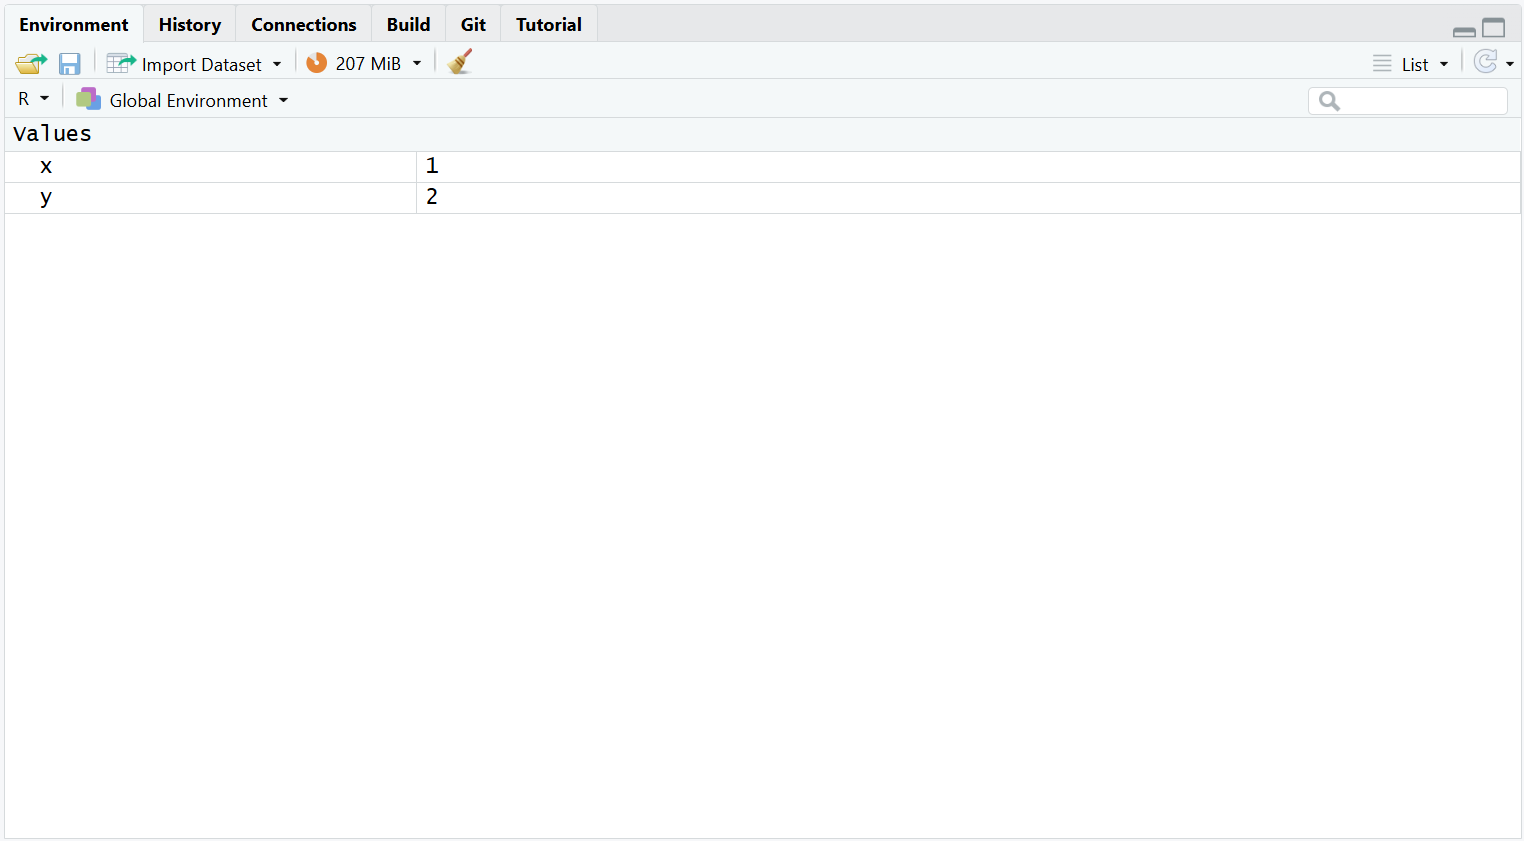
\includegraphics[keepaspectratio]{images/R_screen4.png}}

\textbf{Presenter Notes}: Here you can see an example of how an object
appears in the Environment pane in RStudio.\\
Whenever you create an object using the assignment arrow, R stores it
here. In this example, you can see the object name, along with its value
and type.\\
This is very useful because it allows you to keep track of everything
you have created during your session. Instead of recalculating something
again, you can simply reuse the object from the Environment.\\
As you start working more with R, this pane will become your overview of
what is currently stored in memory.

\textbf{Instructor Notes}: Point students' attention directly to the
Environment pane on their own screens if available. Briefly explain how
objects may change or accumulate as they run more code. Avoid going into
memory management details at this stage.

\textbf{Accessibility Tips}: Verbally describe what is visible in the
screenshot for students who cannot see it clearly. Allow extra time for
learners to locate the Environment pane on their own interface.

\begin{center}\rule{0.5\linewidth}{0.5pt}\end{center}

\subsection{Practical exercise 4}\label{practical-exercise-4}

Try following the example and create your objects!

\begin{itemize}
\tightlist
\item[$\square$]
  Assign the value 4 to \texttt{x}.
\item[$\square$]
  Assign the value 5 to \texttt{y}.
\item[$\square$]
  Run the line(s) and check out your new objects in the Environment
  pane.
\end{itemize}

\textbf{Presenter Notes}: Let's assign some values to objects. Remember
the placement matters: the variable goes in-front of the arrow and the
value goes behind. Run this line to see how the object appears in your
Environment- this also helps you keep track of all the objects you
create.

\begin{center}\rule{0.5\linewidth}{0.5pt}\end{center}

\subsection{Objects and assignments}\label{objects-and-assignments}

\textbf{Okay, I made objects\ldots{} what now?}

\begin{itemize}
\tightlist
\item
  Assigning objects helps organize your values
\item
  Call on them and use specific objects in new operations
\end{itemize}

\begin{Shaded}
\begin{Highlighting}[]
\NormalTok{x }\OtherTok{\textless{}{-}} \DecValTok{1}
\NormalTok{y }\OtherTok{\textless{}{-}} \DecValTok{2}

\CommentTok{\# In a previous slide, we assigned values to the objects}

\CommentTok{\# Now, let\textquotesingle{}s call on the objects and add them together}
\NormalTok{x }\SpecialCharTok{+}\NormalTok{ y}
\end{Highlighting}
\end{Shaded}

\begin{verbatim}
[1] 3
\end{verbatim}

\textbf{Presenter notes}: Once you assign a value to an object, you
don't have to keep remembering or retyping that value every time. You
can just call the object name and use it in your calculations, which
makes your code cleaner and much easier to work with. In the example, we
see that we can call on and perform operations with x and y since we
previously assigned values to those objects.

\begin{center}\rule{0.5\linewidth}{0.5pt}\end{center}

\subsection{Practical exercise 5}\label{practical-exercise-5}

Let's use the objects in a new operation:

\begin{itemize}
\tightlist
\item[$\square$]
  Re-assign the \texttt{x} object with the value \texttt{6}.
\item[$\square$]
  Copy the following to your R Script:
\end{itemize}

\begin{Shaded}
\begin{Highlighting}[]
\NormalTok{x }\SpecialCharTok{+}\NormalTok{ y}
\end{Highlighting}
\end{Shaded}

\begin{itemize}
\tightlist
\item[$\square$]
  Run the line and see what happens.
\end{itemize}

\begin{tcolorbox}[enhanced jigsaw, arc=.35mm, bottomrule=.15mm, bottomtitle=1mm, breakable, colback=white, colbacktitle=quarto-callout-tip-color!10!white, colframe=quarto-callout-tip-color-frame, coltitle=black, left=2mm, leftrule=.75mm, opacityback=0, opacitybacktitle=0.6, rightrule=.15mm, title=\textcolor{quarto-callout-tip-color}{\faLightbulb}\hspace{0.5em}{Object reassignment}, titlerule=0mm, toprule=.15mm, toptitle=1mm]

When you reuse an object name and assign it a new value, R overwrites
the previous value.

\end{tcolorbox}

\textbf{Presenter Notes}: Let's put this to practice by using our
objects in an operation. But first, we will reassign object \texttt{x}.
We will see that if you assign a new value to the same object name, it
simply overwrites the old one. So if x was 4 and is now re-assigned as
\texttt{x\ \textless{}-\ 6}, the value is now 6. R always uses the most
recent assignment. When we complete this practical exercise what do we
observe about object \texttt{x}?

\textbf{Instructor Notes}: It is an important point to make that you can
re-assign objects with new values. Suggestion: Propose the question
``\emph{Why would we want to overwrite objects with new values?}''.

Possible answer: This is a useful feature to avoid cluttering of
objects- knowing that you can simply swap out the value of an object
instead of creating a new object altogether.

\begin{center}\rule{0.5\linewidth}{0.5pt}\end{center}

\section{Functions}\label{functions}

\begin{center}\rule{0.5\linewidth}{0.5pt}\end{center}

\subsection{What is a function?}\label{what-is-a-function}

\begin{itemize}
\tightlist
\item
  A \textbf{function} is a reusable block of code that performs a
  specific task.
\item
  You provide input values (\textbf{arguments}), and R returns an
  \textbf{output} based on internal operations.
\item
  Analogous to a mathematical function:

  \begin{itemize}
  \tightlist
  \item
    If \texttt{f(x)\ =\ 2\ *\ x}, then inputting \texttt{x\ =\ 3}
    returns \texttt{6}.
  \end{itemize}
\item
  Every function has a unique name, followed by parentheses \texttt{()},
  such as \texttt{sum()}.
\end{itemize}

\begin{Shaded}
\begin{Highlighting}[]
\CommentTok{\# Example of a function taking multiple inputs}
\FunctionTok{sum}\NormalTok{(}\DecValTok{1}\NormalTok{, }\DecValTok{2}\NormalTok{, }\DecValTok{3}\NormalTok{, }\DecValTok{4}\NormalTok{)}
\end{Highlighting}
\end{Shaded}

\textbf{Presenter Notes}: Now that we know how to store data in our
working directory, let's talk about how to manipulate it. A function is
basically a recipe. You put ingredients in---these are called
arguments---and the function gives you a finished dish as output. It
saves us from writing complex mathematical formulas from scratch.

\textbf{Instructor Notes}: Emphasize the syntax: the function name is
always immediately followed by parentheses. This is how R distinguishes
a function from an object.

\begin{center}\rule{0.5\linewidth}{0.5pt}\end{center}

\subsection{\texorpdfstring{The \texttt{c()}
function}{The c() function}}\label{the-c-function}

\begin{itemize}
\tightlist
\item
  \textbf{Group items with the \texttt{c()} function} to manipulate
  multiple items at once.
\end{itemize}

\begin{Shaded}
\begin{Highlighting}[]
\CommentTok{\# Example 1: Combine four numbers into one object}
\NormalTok{age }\OtherTok{\textless{}{-}} \FunctionTok{c}\NormalTok{(}\DecValTok{19}\NormalTok{, }\DecValTok{20}\NormalTok{, }\DecValTok{21}\NormalTok{)}

\CommentTok{\# Now we can apply a function to the entire group}
\FunctionTok{sum}\NormalTok{(age)}
\end{Highlighting}
\end{Shaded}

\begin{verbatim}
[1] 60
\end{verbatim}

\begin{Shaded}
\begin{Highlighting}[]
\CommentTok{\# Example 2: Combine four character values into one object}
\NormalTok{food }\OtherTok{\textless{}{-}} \FunctionTok{c}\NormalTok{(}\StringTok{"Pizza"}\NormalTok{, }\StringTok{"Pasta"}\NormalTok{, }\StringTok{"Burger"}\NormalTok{, }\StringTok{"Pasta"}\NormalTok{)}

\CommentTok{\# Now we can organize all the items in this object in a frequency table}
\FunctionTok{table}\NormalTok{(food)}
\end{Highlighting}
\end{Shaded}

\begin{verbatim}
food
Burger  Pasta  Pizza 
     1      2      1 
\end{verbatim}

\textbf{Presenter Notes}: Before we look at more functions, we need to
know one very useful function: the letter `c'. It stands for combine.
Grouping items together allows us to work with groups of information at
a time.

Let's look at the first example. First we will group a series of numbers
and assign it to the object ``age''. Now, whenever we call on ``age'',
we are calling on this group of numbers instead of just one number. So,
if we want to calculate the sum of all the numbers, instead of writing
out each number, we just run the \texttt{sum} operation on the ``age''
object.

In the second example, we first use the c() function to group several
text values together into a vector. Because these are character values,
mathematical operations such as \texttt{sum(food)} do not make sense and
will return an error. However, we can use functions such as
\texttt{table()} to count how often each item appears in the object
``food''.

\begin{center}\rule{0.5\linewidth}{0.5pt}\end{center}

\subsection{Common built-in functions:
Numeric}\label{common-built-in-functions-numeric}

R comes with many built-in \textbf{numeric} functions:

{\def\LTcaptype{none} % do not increment counter
\begin{longtable}[]{@{}lll@{}}
\toprule\noalign{}
Function & What it does & \\
\midrule\noalign{}
\endhead
\bottomrule\noalign{}
\endlastfoot
\texttt{sum()} & Adds all values together & \\
\texttt{mean()} & Calculates the arithmetic mean (average) & \\
\texttt{sd()} & Calculates the standard deviation & \\
\texttt{exp()} & Calculates the exponential function (\(e^x\)) & \\
\texttt{round()} & Rounds a number & \\
\end{longtable}
}

\textbf{Presenter Notes}: Here are some of the most common mathematical
and statistical functions you will use in R when working with numerical
values. They do exactly what their names suggest. For example,
\texttt{sd()} calculates the standard deviation, and \texttt{exp()}
calculates the exponential.

\begin{center}\rule{0.5\linewidth}{0.5pt}\end{center}

\subsection{Practical exercise 6}\label{practical-exercise-6}

\begin{itemize}
\tightlist
\item[$\square$]
  Combine the numbers \texttt{4.4}, \texttt{14}, \texttt{5.26}, and
  \texttt{26} and assign it to an object named ``\texttt{numbers}''
\item[$\square$]
  Try out the functions \texttt{sum()}, \texttt{mean()}, and
  \texttt{sd()} using the object ``\texttt{numbers}'' as the argument
  and inspect the output
\end{itemize}

\textbf{Presenter Notes}: Let's test out the \texttt{c()} function to
group some values into an object and then run some numerical operations.
First we will group a series of numbers and assign it to the object
``numbers''. Then we can call on this object and run some numerical
functions.

\textbf{Instructor Notes}: Give learners about 5-7 minutes. Walk around
to ensure they are properly using the \texttt{c()} function to create
the vector. A common beginner mistake is typing
\texttt{mean(4.4,\ 14,\ 5.26,\ 26)} directly, which will not work as
expected because \texttt{mean()} only calculates the mean of the first
argument if they aren't combined into a vector first.

\begin{center}\rule{0.5\linewidth}{0.5pt}\end{center}

\subsection{Common built-in functions:
Character}\label{common-built-in-functions-character}

R also comes with many built-in \textbf{character} functions:

{\def\LTcaptype{none} % do not increment counter
\begin{longtable}[]{@{}ll@{}}
\toprule\noalign{}
Function & What it does \\
\midrule\noalign{}
\endhead
\bottomrule\noalign{}
\endlastfoot
\texttt{sort()} & Sort values in alphabetical order \\
\texttt{unique()} & Shows the unique values in the set \\
\texttt{table()} & Counts the values in a table \\
\texttt{toupper()} & Transforms all the letters to uppercase \\
\texttt{tolower()} & Transforms all the letters to lowercase \\
\end{longtable}
}

\textbf{Presenter Notes}: As we saw in the example, we can group and
work with multiple character values as well. Here are some of the
built-in functions that allow us to work with these.

\begin{center}\rule{0.5\linewidth}{0.5pt}\end{center}

\subsection{Function arguments}\label{function-arguments}

Most functions take multiple arguments (\textbf{inputs}).

\begin{itemize}
\tightlist
\item
  Arguments are the pieces of information a function needs to
  \textbf{carry out an operation}.
\item
  Different functions expect different types and numbers of arguments,
  and the \textbf{output} of a function often \textbf{depends on the
  arguments} that are supplied.
\item
  It might look something like this:
  \texttt{function\_name(argument1\ =\ x,\ argument2\ =\ y)}
\end{itemize}

\begin{tcolorbox}[enhanced jigsaw, arc=.35mm, bottomrule=.15mm, bottomtitle=1mm, breakable, colback=white, colbacktitle=quarto-callout-note-color!10!white, colframe=quarto-callout-note-color-frame, coltitle=black, left=2mm, leftrule=.75mm, opacityback=0, opacitybacktitle=0.6, rightrule=.15mm, title=\textcolor{quarto-callout-note-color}{\faInfo}\hspace{0.5em}{Do all functions need multiple arguments?}, titlerule=0mm, toprule=.15mm, toptitle=1mm]

No, not all functions need multiple arguments, but for some, it is
required.

\end{tcolorbox}

\textbf{Presenter Notes}: Functions often need information to work with,
and that information is provided through arguments, or inputs. Think of
a function as having two parts: outside the parentheses is \emph{what
you want R to do}, while inside the parentheses is \emph{what you want R
to do it with}. For example, in \texttt{mean(x)}, mean tells R to
calculate an average, and \texttt{x} tells it which data to calculate
the average from. Some functions only need one argument, while others
can take several depending on the task.

\textbf{Instructor Notes}: Some functions need more than one piece of
information. Up to this point, learners have seen functions being used,
but may not have thought about what goes inside the parentheses.
Emphasize that the values inside the parentheses are called arguments
and that they provide the information the function needs to work.
Different functions need different information, so the arguments will
vary depending on the task.

\begin{center}\rule{0.5\linewidth}{0.5pt}\end{center}

\subsection{Function arguments}\label{function-arguments-1}

Example: The \texttt{round()} function

\begin{itemize}
\tightlist
\item
  This function uses two arguments: It approximates a number
  (\textbf{x}) to a specified amount of decimal places
  (\textbf{digits}).
\item
  You can provide arguments by position or by name.
\end{itemize}

\begin{Shaded}
\begin{Highlighting}[]
\CommentTok{\# By position (R assumes the first number is x, the second is digits)}
\FunctionTok{round}\NormalTok{(}\FloatTok{3.14159}\NormalTok{, }\DecValTok{2}\NormalTok{)}

\CommentTok{\# By name (explicitly telling R which argument is which)}
\FunctionTok{round}\NormalTok{(}\AttributeTok{x =} \FloatTok{3.14159}\NormalTok{, }\AttributeTok{digits =} \DecValTok{2}\NormalTok{)}
\end{Highlighting}
\end{Shaded}

\begin{tcolorbox}[enhanced jigsaw, arc=.35mm, bottomrule=.15mm, bottomtitle=1mm, breakable, colback=white, colbacktitle=quarto-callout-tip-color!10!white, colframe=quarto-callout-tip-color-frame, coltitle=black, left=2mm, leftrule=.75mm, opacityback=0, opacitybacktitle=0.6, rightrule=.15mm, title=\textcolor{quarto-callout-tip-color}{\faLightbulb}\hspace{0.5em}{Naming your arguments makes your code easier to read!}, titlerule=0mm, toprule=.15mm, toptitle=1mm]

If you name the arguments (using the names ``x'' and ``digits''), the
order does not matter: \texttt{round(digits\ =\ 2,\ x\ =\ 3.14159)}
works identically.

\end{tcolorbox}

\textbf{Presenter Notes}: For instance, to round a number, R needs to
know two things: what number to round and how many decimals to keep. You
can just type the numbers in the right order, but explicitly naming the
arguments, like writing \texttt{digits\ =\ 2}, is highly recommended
because it makes your script much easier to understand when you read it
a month later.

\begin{center}\rule{0.5\linewidth}{0.5pt}\end{center}

\subsection{Practical exercise 7}\label{practical-exercise-7}

\begin{itemize}
\tightlist
\item[$\square$]
  Assign a ``\texttt{my\_number}'' object using \texttt{2.4637}
\item[$\square$]
  Try out the function \texttt{round()} using ``\texttt{my\_number}''
  and approximating to 3 decimal places.
\end{itemize}

\begin{tcolorbox}[enhanced jigsaw, arc=.35mm, bottomrule=.15mm, bottomtitle=1mm, breakable, colback=white, colbacktitle=quarto-callout-tip-color!10!white, colframe=quarto-callout-tip-color-frame, coltitle=black, left=2mm, leftrule=.75mm, opacityback=0, opacitybacktitle=0.6, rightrule=.15mm, title=\textcolor{quarto-callout-tip-color}{\faLightbulb}\hspace{0.5em}{Ignoring the \textbf{digits} argument}, titlerule=0mm, toprule=.15mm, toptitle=1mm]

If you are curious, try running the \texttt{round()} function without
specifying the \texttt{digits\ =} argument. What happens? Why might that
be?

\end{tcolorbox}

\textbf{Presenter Notes}: Next, let's practice specifying arguments
using the \texttt{round()} function. We can reuse the ``my\_number''
object name, simply re-assign it with a new number. Then, follow the
order from the previous slide on how to specify the arguments.

\textbf{Instructor Notes}: It may be confusing to remember the order and
to know what goes where.

\begin{center}\rule{0.5\linewidth}{0.5pt}\end{center}

\subsection{Pre-break quiz}\label{pre-break-quiz}

\textbf{Presenter Notes}: Before we head into the break, let's do a
quick check-in to see how things are going so far. The questions are
designed to help you reflect on your current understanding of R,
RStudio, and the key ideas we've covered in this first part of the
session.

\textbf{Instructor Notes}: Use this pre-break survey to gauge learners'
understanding of the submodule's core concepts.

\begin{itemize}
\item
  If more than 80\% of learners select the correct answer, briefly
  confirm the correct response and continue.
\item
  If fewer than 80\% answer correctly, give learners 1--2 minutes to
  discuss their reasoning with a partner before re-running the question.
  If results improve above 80\%, continue; otherwise, explain the
  correct answer and address common misunderstandings.
\item
  If a large portion of learners select the same distractor answer,
  pause to discuss why that option may seem plausible and clarify the
  misconception.
\end{itemize}

\textbf{Accessibility Tip}: This activity is designed for synchronous
teaching settings and may be skipped or adapted if needed.

\begin{center}\rule{0.5\linewidth}{0.5pt}\end{center}

\textbf{1. What does the \texttt{\#} symbol do in R?}

\begin{enumerate}
\def\labelenumi{\alph{enumi}.}
\tightlist
\item
  Runs the code\\
\item
  Creates a variable\\
\item
  Starts a comment\\
\item
  Multiplies numbers
\end{enumerate}

\textbf{Instructor notes}: The answer for this question is c

\begin{center}\rule{0.5\linewidth}{0.5pt}\end{center}

\textbf{2. What happens when you ``run'' code in R?}

\begin{enumerate}
\def\labelenumi{\alph{enumi}.}
\tightlist
\item
  The code is deleted\\
\item
  R executes the command\\
\item
  The code becomes a comment\\
\item
  RStudio closes automatically
\end{enumerate}

\textbf{Instructor notes}: The answer for this question is b

\begin{center}\rule{0.5\linewidth}{0.5pt}\end{center}

\textbf{3. What will R return for this comparison?}

\texttt{49\ \textless{}\ 50}

\begin{enumerate}
\def\labelenumi{\alph{enumi}.}
\tightlist
\item
  TRUE
\item
  FALSE
\item
  49
\item
  ERROR
\end{enumerate}

\textbf{Instructor notes}: The answer for this question is a

\begin{center}\rule{0.5\linewidth}{0.5pt}\end{center}

\textbf{4. Which of the following is a character value in R?}

\begin{enumerate}
\def\labelenumi{\alph{enumi}.}
\tightlist
\item
  TRUE
\item
  5
\item
  ``hello''
\item
  4.2
\end{enumerate}

\textbf{Instructor notes}: The answer for this question is c

\begin{center}\rule{0.5\linewidth}{0.5pt}\end{center}

\textbf{5. Why does the following produce an error?}

\texttt{4\ +\ "five"}

\begin{enumerate}
\def\labelenumi{\alph{enumi}.}
\tightlist
\item
  ``five'' is a logical value
\item
  The quotation marks are incorrect
\item
  4 is not numeric
\item
  R cannot numerically add different data types together
\end{enumerate}

\textbf{Instructor notes}: The answer for this question is d

\begin{center}\rule{0.5\linewidth}{0.5pt}\end{center}

\section{Break! 15 minutes}\label{break-15-minutes}

\begin{center}\rule{0.5\linewidth}{0.5pt}\end{center}

\subsection{Post-break quiz
discussion}\label{post-break-quiz-discussion}

What do we see in the results?

\textbf{Presenter Notes}: Let us have a look at these results.

\textbf{Instructor Notes}: Briefly examine the answers given to each
question interactively with the group. Use visuals from the survey to
highlight specific answers. Serves to clarify concepts and aspects that
are not yet understood. Highlight specific answers given during the
survey.

\textbf{Accessibility Tip}: Have people work in pairs if someone did not
bring their phone/does not have a phone. This survey also cannot be
completed in an asynchronous setting.

\begin{center}\rule{0.5\linewidth}{0.5pt}\end{center}

\subsection{The Help function}\label{the-help-function}

\textbf{Do I have to memorize all of the functions and arguments?}

\begin{itemize}
\tightlist
\item
  \textbf{No!}

  \begin{itemize}
  \tightlist
  \item
    There is no need to memorize functions and their arguments.
  \item
    You will \textbf{remember} the ones you use frequently
    \textbf{through practice}.
  \end{itemize}
\item
  When you need to understand how a function works, what inputs it
  needs, or what its defaults are, you can consult the \textbf{Help
  Function}.
\end{itemize}

\textbf{Presenter Notes}: A common worry when learning a programming
language is feeling like you have to memorize a dictionary of functions.
Please don't! Even advanced programmers look up functions every single
day. The more you use certain functions, the more naturally they will
come to you. For everything else, R has a built-in manual called the
Help Function.

\textbf{Instructor Notes}: Normalize the act of looking things up. You
can mention that googling errors or looking at documentation is 80\% of
programming.

\begin{center}\rule{0.5\linewidth}{0.5pt}\end{center}

\subsection{How to access Help in R}\label{how-to-access-help-in-r}

There are two main ways to look up a function.

\textbf{Method 1: Using the Console}

\begin{itemize}
\tightlist
\item
  Type a question mark \texttt{?} into the console immediately followed
  by the function name and press Enter.
\end{itemize}

\begin{Shaded}
\begin{Highlighting}[]
\CommentTok{\# Example: Getting help with using the round() function}
\NormalTok{?round}
\end{Highlighting}
\end{Shaded}

\textbf{Presenter Notes}: There are two simple ways to access help for a
function in R. The first is by using a shortcut in the Console. Simply
type a question mark (?) immediately before the function name without
parentheses and press Enter. For example, typing \texttt{?round} opens
the help page for the \texttt{round()} function, where you can find
information about what it does, its arguments, and examples of how to
use it.

\textbf{Instructor Notes}: Emphasize that the syntax matters. The
question mark (?) must come before the function name, and parentheses
should not be included. For example, \texttt{?round} is correct, whereas
\texttt{?round()} is not. Encourage students to use this frequently
whenever they are unsure how a function works.

\begin{center}\rule{0.5\linewidth}{0.5pt}\end{center}

\subsection{How to access Help in R}\label{how-to-access-help-in-r-1}

\textbf{Method 2: Using the Help Tab}

\begin{itemize}
\tightlist
\item
  Navigate to the \textbf{Help} tab in the bottom right pane of RStudio
  and type the function name into the search bar.
\end{itemize}

\pandocbounded{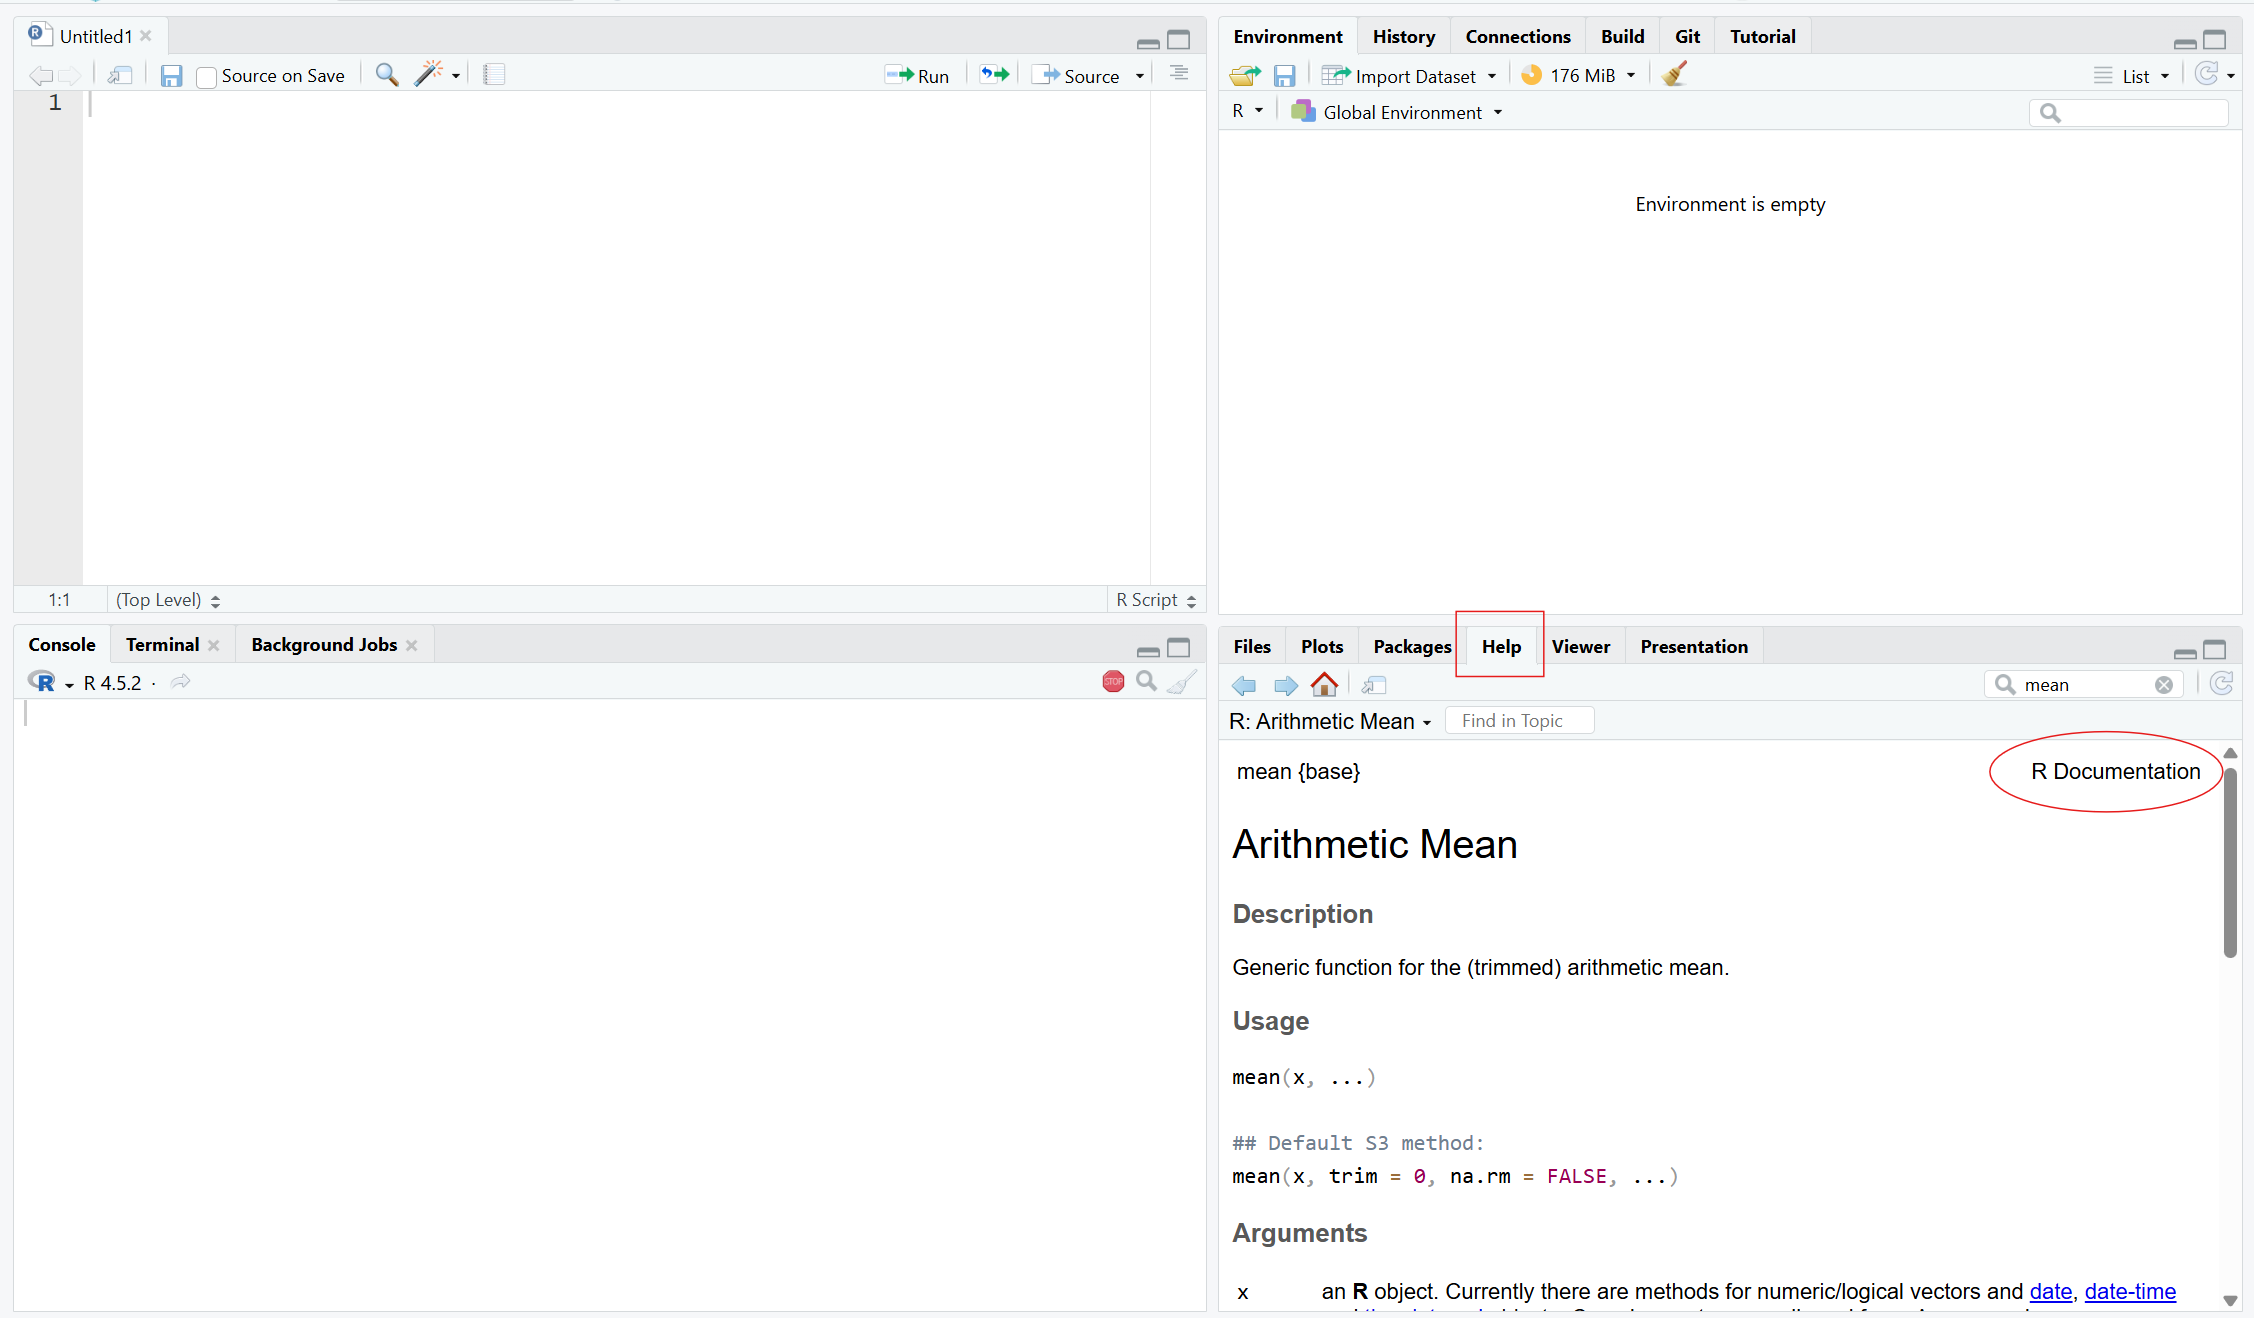
\includegraphics[keepaspectratio]{images/help_search_bar.png}}

\textbf{Presenter Notes}: Alternatively, you can use the search bar in
the Help tab located in the bottom right pane of RStudio. Here, you can
type directly in the \emph{search bar} to look up the name of the
function.

\begin{center}\rule{0.5\linewidth}{0.5pt}\end{center}

\subsection{Reading the documentation}\label{reading-the-documentation}

Help pages can look intimidating, but you only need to focus on a few
key sections:

\begin{itemize}
\tightlist
\item
  \textbf{Description:} A brief summary of what the function does.
\item
  \textbf{Usage:} Shows the function with all arguments. This is where
  you see \emph{default values}.
\item
  \textbf{Arguments:} Detailed explanations of what each input to the
  function should look like.
\end{itemize}

\textbf{Presenter Notes}: The documentation might look overwhelming at
first because it uses technical terms. As a start, focus on the
``Usage'' and ``Arguments'' sections.

\begin{center}\rule{0.5\linewidth}{0.5pt}\end{center}

\subsection{Reading the
documentation}\label{reading-the-documentation-1}

Example: For the \texttt{sort()} function we can see that it can also
use character vectors or values as input and orders them.

\pandocbounded{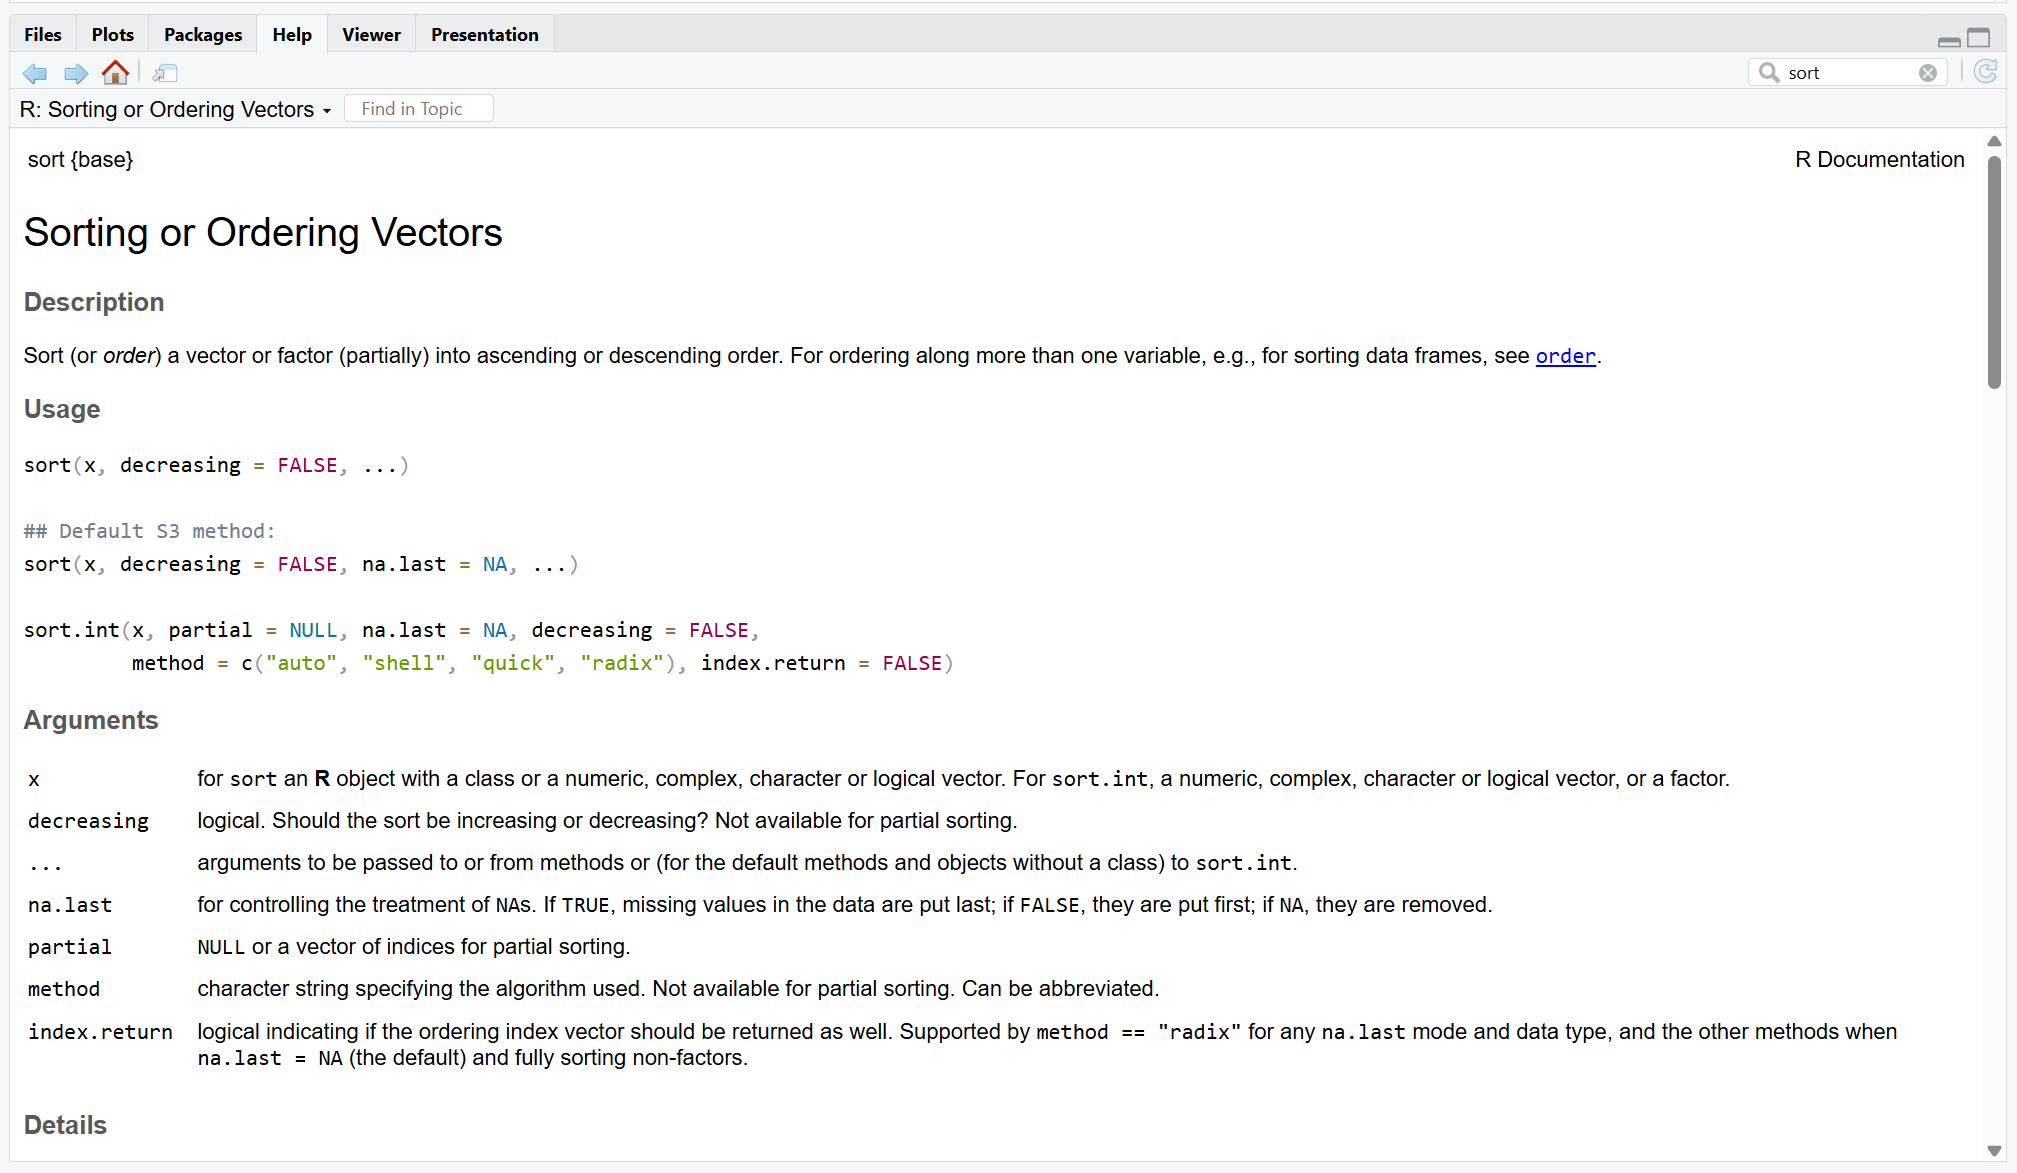
\includegraphics[keepaspectratio]{images/help_sort_docs.png}}

\textbf{Presenter Notes}: In this example, we use the documentation for
\texttt{sort()} to see that the function can work not only with numbers,
but also with character values. By looking at the \emph{Usage} and
\emph{Arguments} sections, we can identify that the first argument,
\texttt{x}, is the object(s) we want to sort. We can also see that the
argument \texttt{decreasing\ =\ FALSE} means that, by default, the
values are sorted in ascending order (A to Z for text). This illustrates
how the documentation can help us understand both what a function does
and how we can customize its behavior.

\begin{center}\rule{0.5\linewidth}{0.5pt}\end{center}

\subsection{Practical exercise 8}\label{practical-exercise-8}

\begin{itemize}
\tightlist
\item[$\square$]
  Type \texttt{?sort} in the \textbf{Console} and press Enter.
\item[$\square$]
  Look at the \textbf{Usage} and \textbf{Arguments} sections in the
  documentation that opens in the bottom right pane to see which inputs
  the function accepts.
\item[$\square$]
  Put the following as the input for the function:
\end{itemize}

\begin{Shaded}
\begin{Highlighting}[]
\NormalTok{c("Tim", "Tom", "Anna", "Pizza", "Burger", "Pasta")}
\end{Highlighting}
\end{Shaded}

\begin{itemize}
\tightlist
\item[$\square$]
  Read the \textbf{Arguments} to figure out what must be included to put
  the words in \emph{reverse alphabetical} order
\end{itemize}

\begin{tcolorbox}[enhanced jigsaw, arc=.35mm, bottomrule=.15mm, bottomtitle=1mm, breakable, colback=white, colbacktitle=quarto-callout-note-color!10!white, colframe=quarto-callout-note-color-frame, coltitle=black, left=2mm, leftrule=.75mm, opacityback=0, opacitybacktitle=0.6, rightrule=.15mm, title=\textcolor{quarto-callout-note-color}{\faInfo}\hspace{0.5em}{Is reverse alphabetical order increasing or decreasing?}, titlerule=0mm, toprule=.15mm, toptitle=1mm]

Reverse alphabetical order means arranging items from \textbf{Z to A}.
This means that the order is \emph{decreasing}.

\end{tcolorbox}

\textbf{Presenter Notes}: Let's try this exercise to become more
comfortable navigating R's documentation. Don't worry if some of the
terminology seems unfamiliar. Focus on identifying the important
information: what the function does, what inputs it accepts, and how to
change its behavior.

\textbf{Instructor Notes}: This exercise can be tricky since the Help
documentation has a lot of information that can be confusing to
learners. It's important to let them know that not every piece of
information is relevant and just to focus on the pieces they need to
complete the exercise.

Some issues you might encounter: - Missing parentheses () around ALL the
arguments. - Missing comma , after the parentheses that hold the
character values. - Must use the \texttt{decreasing\ =\ TRUE/FALSE}
argument (in this case, it must be \texttt{decreasing\ =\ TRUE}). Using
\texttt{increasing\ =\ FALSE} would NOT work. - They may feel the need
to include the other arguments they see in the document but this is
unnecessary.

\begin{center}\rule{0.5\linewidth}{0.5pt}\end{center}

\section{Vectors, lists, and data
frames}\label{vectors-lists-and-data-frames}

\begin{center}\rule{0.5\linewidth}{0.5pt}\end{center}

\subsection{Data structures in R}\label{data-structures-in-r}

\begin{itemize}
\item
  Collections of values are called \textbf{data}
\item
  R provides ways to store data in different \textbf{data structures}:

  \begin{itemize}
  \tightlist
  \item
    \textbf{Vectors}
  \item
    \textbf{Lists}
  \item
    \textbf{Dataframes}
  \end{itemize}
\end{itemize}

\textbf{Presenter Notes}: So far, we have mostly worked with single
values. Most of the time, we are interested in a collection of values
rather than a single value, allowing us to work with many observations
at once. R provides different data structures to help us organize and
work with collections of data.

\textbf{Instructor Notes}: This next section introduce several new
technical concepts that beginners often confuse. Regularly remind
students what vectors, lists, and data frames are as they appear, and
briefly recap the differences before introducing the next concept.

\begin{center}\rule{0.5\linewidth}{0.5pt}\end{center}

\subsection{Vectors}\label{vectors}

\textbf{What does a vector do?} Stores multiple values in an object.

\begin{itemize}
\tightlist
\item
  It is a one-dimensional collection of data
\item
  Useful for storing scores, ages, measurements, names, and more
\end{itemize}

Example:

\begin{Shaded}
\begin{Highlighting}[]
\NormalTok{scores }\OtherTok{\textless{}{-}} \FunctionTok{c}\NormalTok{(}\DecValTok{75}\NormalTok{, }\DecValTok{82}\NormalTok{, }\DecValTok{91}\NormalTok{, }\DecValTok{68}\NormalTok{)}
\end{Highlighting}
\end{Shaded}

\begin{tcolorbox}[enhanced jigsaw, arc=.35mm, bottomrule=.15mm, bottomtitle=1mm, breakable, colback=white, colbacktitle=quarto-callout-tip-color!10!white, colframe=quarto-callout-tip-color-frame, coltitle=black, left=2mm, leftrule=.75mm, opacityback=0, opacitybacktitle=0.6, rightrule=.15mm, title=\textcolor{quarto-callout-tip-color}{\faLightbulb}\hspace{0.5em}{Vectors and data type}, titlerule=0mm, toprule=.15mm, toptitle=1mm]

What do you notice about the values in the vector stored in
\texttt{scores}? All values in a vector should be of the same data type.

\end{tcolorbox}

\textbf{Presenter Notes}: A vector is one of the most common data
structures in R. Think of it as a container that stores many related
values under a single name. Instead of creating separate objects for
each score, we can store them together in one vector. Important to note
is that vectors only contain one data type, e.g., all values in a vector
are numeric, or all values are character type.

\textbf{Instructor Notes}: For added clarity, you can emphasize that, in
the example, ``\texttt{c(75,82,\ 91,\ 68)}'' is the vector and
``scores'' is just the object name in which the vector is stored.

\begin{center}\rule{0.5\linewidth}{0.5pt}\end{center}

\subsection{Practical exercise 9}\label{practical-exercise-9}

\begin{itemize}
\item[$\square$]
  Create a vector containing the numbers \texttt{19}, \texttt{20}, and
  \texttt{21} and assign it to an object called ``\texttt{age}''.
\item[$\square$]
  Create a vector containing the names \texttt{Tim}, \texttt{Tom}, and
  \texttt{Anna} and assign it to an object called ``\texttt{name}''.
\item[$\square$]
  Create a vector containing the foods \texttt{Pizza}, \texttt{Burger},
  and \texttt{Pasta} and assign it to an object called
  ``\texttt{food}''.
\end{itemize}

\begin{tcolorbox}[enhanced jigsaw, arc=.35mm, bottomrule=.15mm, bottomtitle=1mm, breakable, colback=white, colbacktitle=quarto-callout-tip-color!10!white, colframe=quarto-callout-tip-color-frame, coltitle=black, left=2mm, leftrule=.75mm, opacityback=0, opacitybacktitle=0.6, rightrule=.15mm, title=\textcolor{quarto-callout-tip-color}{\faLightbulb}\hspace{0.5em}{Character data type}, titlerule=0mm, toprule=.15mm, toptitle=1mm]

Reminder: character data types need to be wrapped in quotation marks
\texttt{"\ "}.

\end{tcolorbox}

\textbf{Presenter Notes}: Let's try making some vectors of our own using
both numerical and word data types. But remember, for each vector, just
use one datatype. At the end of this exercise, you should have two
separate vectors each assigned to a different object.

\textbf{Instructor Notes}: Here are the solutions:

\begin{Shaded}
\begin{Highlighting}[]
\NormalTok{age }\OtherTok{\textless{}{-}} \FunctionTok{c}\NormalTok{(}\DecValTok{19}\NormalTok{, }\DecValTok{20}\NormalTok{, }\DecValTok{21}\NormalTok{)}
\NormalTok{name }\OtherTok{\textless{}{-}} \FunctionTok{c}\NormalTok{(}\StringTok{"Tim"}\NormalTok{, }\StringTok{"Tom"}\NormalTok{, }\StringTok{"Anna"}\NormalTok{)}
\NormalTok{food }\OtherTok{\textless{}{-}} \FunctionTok{c}\NormalTok{(}\StringTok{"Pizza"}\NormalTok{, }\StringTok{"Burger"}\NormalTok{, }\StringTok{"Pasta"}\NormalTok{)}
\end{Highlighting}
\end{Shaded}

Though it is added as a callout-tip, still be mindful that a common
mistake is forgetting to wrap the character and word data in quotation
marks. This will lead to an error.

\begin{center}\rule{0.5\linewidth}{0.5pt}\end{center}

\subsection{Lists}\label{lists}

\textbf{What does a list do?} Stores different types of data together.

\begin{itemize}
\tightlist
\item
  It is also one-dimensional
\item
  \emph{But}, unlike vectors, it can contain \textbf{different data
  types} (e.g., numeric, character\ldots)
\end{itemize}

Example for a list:

\begin{Shaded}
\begin{Highlighting}[]
\NormalTok{student }\OtherTok{\textless{}{-}} \FunctionTok{list}\NormalTok{(}\StringTok{"Alex"}\NormalTok{, }\DecValTok{21}\NormalTok{, }\ConstantTok{TRUE}\NormalTok{)}
\end{Highlighting}
\end{Shaded}

\textbf{Presenter Notes}: Unlike vectors, lists can contain different
types of information. For example, text, numbers, and logical values can
all be stored together. We won't use lists much in this introductory
session, but it's useful to know they exist.

\textbf{Instructor Notes}: Since they are quite similar, it can be
useful here to note that both lists and vectors group together pieces of
information but the difference is that lists can contain different
datatypes.

Also, for added clarity, you can mention that, in this example,
``\texttt{list("Alex",\ 21,\ TRUE)}'' is the list and ``student'' is
simply the object name in which the list is stored or assigned to.

\begin{center}\rule{0.5\linewidth}{0.5pt}\end{center}

\subsection{Dataframes}\label{dataframes}

\textbf{What does a dataframe do?} Stores data in rows and columns. - It
is \textbf{two}-dimensional - \textbf{Rows} represent observations,
\textbf{columns} represent variables

{\def\LTcaptype{none} % do not increment counter
\begin{longtable}[]{@{}lll@{}}
\toprule\noalign{}
Name & Age & Food \\
\midrule\noalign{}
\endhead
\bottomrule\noalign{}
\endlastfoot
Tim & 19 & Pizza \\
Tom & 20 & Pizza \\
Anna & 21 & Pasta \\
\end{longtable}
}

\begin{tcolorbox}[enhanced jigsaw, arc=.35mm, bottomrule=.15mm, bottomtitle=1mm, breakable, colback=white, colbacktitle=quarto-callout-note-color!10!white, colframe=quarto-callout-note-color-frame, coltitle=black, left=2mm, leftrule=.75mm, opacityback=0, opacitybacktitle=0.6, rightrule=.15mm, title=\textcolor{quarto-callout-note-color}{\faInfo}\hspace{0.5em}{Look familiar?}, titlerule=0mm, toprule=.15mm, toptitle=1mm]

Think of a dataframe like a spreadsheet. The top row is like the heading
and the information below (within each column) is the observation
corresponding to the heading.

\end{tcolorbox}

\textbf{Presenter Notes}: Dataframes are one of the most important data
structures in R because most datasets are stored this way. If you've
used Excel or any type of spreadsheets before, think of a dataframe as a
table where rows contain observations and columns contain variables.

\textbf{Intructor Notes}: To avoid confusion, use the example to explain
further the breakdown of a dataframe: \texttt{Name} is the observation-
it's what we are interested in finding out. Then each name under it
(\texttt{Tim,\ Tom,\ Anna}) are the variables within this specific
observation.

\begin{center}\rule{0.5\linewidth}{0.5pt}\end{center}

\subsection{Practical exercise 10}\label{practical-exercise-10}

Create a dataframe with the \texttt{data.frame()} function

\begin{itemize}
\tightlist
\item[$\square$]
  Copy the following to combine the vectors you created before into the
  \textbf{dataframe} named ``\texttt{people\_data}''
\end{itemize}

\begin{Shaded}
\begin{Highlighting}[]
\NormalTok{people\_data }\OtherTok{\textless{}{-}} \FunctionTok{data.frame}\NormalTok{(name, age, food)}
\end{Highlighting}
\end{Shaded}

\begin{itemize}
\tightlist
\item[$\square$]
  Call on the dataframe and observe what happens
\end{itemize}

\textbf{Presenter Notes}: Here we're are using the three separate
vectors we created in the previous exercise and combine them them into a
dataframe with the \texttt{data.frame()} function. Notice how each
vector becomes a column in the final table.

\textbf{Instructor Notes}: A concern that you can clear up here is
confusing the observations in the dataframe with character data types-
when using them in \texttt{data.frame()}, the observations do NOT need
to be wrapped in quotations.

Calling on the dataframe is done by simply typing the object name of the
dataframe (``\texttt{people\_data}'' in this case) in the script (or
Console) and running it.

\begin{center}\rule{0.5\linewidth}{0.5pt}\end{center}

\subsection{Indexing}\label{indexing}

\textbf{What does indexing do?} Allows us to access specific parts of
our data, such as:

\begin{itemize}
\tightlist
\item
  \textbf{Select} individual or multiple values
\item
  \textbf{Access} rows and columns in a dataframe
\end{itemize}

\textbf{Presenter Notes}: Indexing means selecting a specific part of an
object. Instead of viewing all values at once, we can ask R to return
only the piece we need.

\begin{center}\rule{0.5\linewidth}{0.5pt}\end{center}

\subsection{Indexing vectors}\label{indexing-vectors}

Each element in a vector has a position.

\begin{Shaded}
\begin{Highlighting}[]
\NormalTok{age }\OtherTok{\textless{}{-}} \FunctionTok{c}\NormalTok{(}\DecValTok{19}\NormalTok{, }\DecValTok{20}\NormalTok{, }\DecValTok{21}\NormalTok{)}
\end{Highlighting}
\end{Shaded}

{\def\LTcaptype{none} % do not increment counter
\begin{longtable}[]{@{}llll@{}}
\toprule\noalign{}
Position & 1 & 2 & 3 \\
\midrule\noalign{}
\endhead
\bottomrule\noalign{}
\endlastfoot
Value & 19 & 20 & 21 \\
\end{longtable}
}

\textbf{Presenter Notes}: Let's first look at this vector to understand
that each element within that vector has a position. The values are
stored sequentially, so the first value is in position 1, the second in
position 2, and so on.

\begin{center}\rule{0.5\linewidth}{0.5pt}\end{center}

\subsection{Indexing vectors}\label{indexing-vectors-1}

\textbf{Selecting individual values}

\begin{itemize}
\tightlist
\item
  Use \texttt{{[}\ {]}} to call on a value by its position
\end{itemize}

\begin{Shaded}
\begin{Highlighting}[]
\CommentTok{\# Example 1: Calling on the value in position 1 }
\NormalTok{age[}\DecValTok{1}\NormalTok{]}
\end{Highlighting}
\end{Shaded}

\begin{verbatim}
[1] 19
\end{verbatim}

\begin{Shaded}
\begin{Highlighting}[]
\CommentTok{\# Example 2: Calling on the value in position 3}
\NormalTok{age[}\DecValTok{3}\NormalTok{]}
\end{Highlighting}
\end{Shaded}

\begin{verbatim}
[1] 21
\end{verbatim}

\textbf{Presenter Notes}: Now that we know each value has a position
within the vector, we can use this to call on it. The first possible
position that R assigns is 1, so calling on the item in position
``\texttt{1}'', is calling on the first item in the vector. We specify
the position by using the square brackets {[} {]} where number inside
the square brackets refers to the position of the value we want to
retrieve. Let's see this in action with the examples: we first specify
the object (``\texttt{age}'') and then we use the square brackets to
indicate which is position of the items we want (``\texttt{{[}1{]}}'' or
``\texttt{{[}3{]}}'').

\begin{center}\rule{0.5\linewidth}{0.5pt}\end{center}

\subsection{Indexing vectors}\label{indexing-vectors-2}

\textbf{Selecting multiple values}

You can retrieve \textbf{more than one} value at once.

\begin{Shaded}
\begin{Highlighting}[]
\NormalTok{age[}\FunctionTok{c}\NormalTok{(}\DecValTok{1}\NormalTok{,}\DecValTok{3}\NormalTok{)]}
\end{Highlighting}
\end{Shaded}

\begin{verbatim}
[1] 19 21
\end{verbatim}

You can also select a \textbf{range}:

\begin{Shaded}
\begin{Highlighting}[]
\NormalTok{age[}\DecValTok{1}\SpecialCharTok{:}\DecValTok{3}\NormalTok{]}
\end{Highlighting}
\end{Shaded}

\begin{verbatim}
[1] 19 20 21
\end{verbatim}

\textbf{Presenter Notes}: We can also use indexing to select several
positions at the same time. For this, we utilize a comma between the
positions. Additionally, we can use the colon operator to call on a
sequence of positions.

\begin{center}\rule{0.5\linewidth}{0.5pt}\end{center}

\subsection{Indexing dataframes}\label{indexing-dataframes}

\textbf{Accessing rows and columns in a dataframe}

\begin{itemize}
\item
  You can call on values directly from the row and column of data
  frames.
\item
  To use indexing, use \texttt{{[}\ {]}} and follow this general format:

  \begin{itemize}
  \tightlist
  \item
    \texttt{dataframe{[}row,column{]}}
  \end{itemize}
\end{itemize}

\begin{Shaded}
\begin{Highlighting}[]
\CommentTok{\# Example 1: Calling the value in row 1, column 1}
\NormalTok{people\_data[}\DecValTok{1}\NormalTok{, }\DecValTok{1}\NormalTok{]}
\end{Highlighting}
\end{Shaded}

\begin{verbatim}
[1] "Tim"
\end{verbatim}

\begin{Shaded}
\begin{Highlighting}[]
\CommentTok{\# Example 2: Calling the value in row 3, column 2}
\NormalTok{people\_data[}\DecValTok{3}\NormalTok{, }\DecValTok{2}\NormalTok{]}
\end{Highlighting}
\end{Shaded}

\begin{verbatim}
[1] 21
\end{verbatim}

\textbf{Presenter Notes}: Unlike vectors, dataframes are two-dimensional
because they contain both observations (rows) and variables (columns).
This means that when indexing a data frame, we need to specify two
positions: the row position and the column position. Just like vectors,
R assigns positions starting at 1. The columns are numbered from left to
right, so the first column is in position 1, the second column is in
position 2, and so on. Likewise, the rows are numbered from top to
bottom, starting with the first observation \textbf{below the column
headings}. To access a value, we first specify the row (observation) and
then the column (variable).

\begin{center}\rule{0.5\linewidth}{0.5pt}\end{center}

\subsection{Accessing columns by name}\label{accessing-columns-by-name}

Calling values by using just numbers can get confusing.

Luckily, there is a way to call on the values by \textbf{column name}
using the \texttt{\$} operator: \texttt{dataframe\$column\_name}

\begin{itemize}
\tightlist
\item
  Use it to retrieve all values from that specific column
\item
  It is easier to read than using column numbers
\end{itemize}

\begin{Shaded}
\begin{Highlighting}[]
\CommentTok{\# Example: Calling on the "name" column within the "people\_data" data frame}

\NormalTok{people\_data}\SpecialCharTok{$}\NormalTok{name}
\end{Highlighting}
\end{Shaded}

\begin{verbatim}
[1] "Tim"  "Tom"  "Anna"
\end{verbatim}

\textbf{Presenter Notes}: The dollar sign (\texttt{\$}) is a convenient
way to access a column in a data frame. Instead of remembering which
column number contains the information we want, we can simply use the
column's name or header. This makes code easier to read and understand.

\begin{center}\rule{0.5\linewidth}{0.5pt}\end{center}

\subsection{\texorpdfstring{Combining \texttt{\$} and
\texttt{{[}{]}}}{Combining \$ and {[}{]}}}\label{combining-and}

Look at the following example to see how \texttt{\$} and
\texttt{{[}\ {]}} can be used together:

\begin{Shaded}
\begin{Highlighting}[]
\NormalTok{people\_data}\SpecialCharTok{$}\NormalTok{food[}\DecValTok{3}\NormalTok{]}
\end{Highlighting}
\end{Shaded}

\begin{verbatim}
[1] "Pasta"
\end{verbatim}

What does this do?

\begin{enumerate}
\def\labelenumi{\arabic{enumi}.}
\tightlist
\item
  \texttt{\$} selects the \textbf{food} column in the
  \texttt{people\_data} data frame
\item
  \texttt{{[}{]}} gives you the \textbf{third} value
\end{enumerate}

\textbf{Presenter Notes}: This is a very common pattern in R. We first
select a column and then use indexing to retrieve a specific value from
that column. Looking at the example, we first state
\texttt{people\_data} then we use \texttt{\$} to let R know we will be
selecting specific information from this dataframe. Then we specify the
information we want: using the column name, we want to look into the
``food'' column and then, using the square brackets {[} {]}, we specify
we want the third variable in this column.

\begin{center}\rule{0.5\linewidth}{0.5pt}\end{center}

\subsection{Practical exercise 11}\label{practical-exercise-11}

Use \texttt{\$} and \texttt{{[}{]}} accordingly to retrieve the
following information from the the \texttt{people\_data} data frame:

\begin{itemize}
\tightlist
\item[$\square$]
  The first name in the ``name'' column
\item[$\square$]
  The second age in the ``age'' column
\item[$\square$]
  The third food item in the ``food'' column
\end{itemize}

\textbf{Presenter Notes}: Now we'll apply what we've learned about
indexing data frames using column names. For this exercise, the names of
the columns have already been provided for you, so your task is to
retrieve the correct value by combining the appropriate column name with
the correct row position. Remember that you can use either \texttt{\$}
or \texttt{{[}{]}} notation where appropriate.

\textbf{Instructor Notes}: Students commonly make a few mistakes here.
Remind them that column names should not be enclosed in quotation marks
when using the \texttt{\$} operator (e.g., \texttt{people\_data\$name},
not \texttt{people\_data\$"name"}). Also watch for students reversing
the indexing order- the correct syntax is always column name first, then
position within the column:
dataframe\$column\_name{[}column\_position{]}

\begin{center}\rule{0.5\linewidth}{0.5pt}\end{center}

\section{Wrapping Up}\label{wrapping-up}

\begin{center}\rule{0.5\linewidth}{0.5pt}\end{center}

\subsection{Looking into the future}\label{looking-into-the-future}

\begin{enumerate}
\def\labelenumi{\arabic{enumi}.}
\tightlist
\item
  \textbf{Take a minute to think about the following questions, first
  for yourself, then in a pair:}
\end{enumerate}

\begin{itemize}
\item
  Can you identify some \textbf{practical benefits} of using R/RStudio?
\item
  What \textbf{obstacles} do you anticipate in using it consistently?
\item
  How can R/RStudio support you in your \textbf{upcoming projects}?
\end{itemize}

\begin{enumerate}
\def\labelenumi{\arabic{enumi}.}
\setcounter{enumi}{1}
\tightlist
\item
  \textbf{Share your thoughts with the group.}
\end{enumerate}

\textbf{Presenter Notes}: To wrap up, let's take a moment to bring
everything together and think about how this connects to your own work
going forward.First, take about one minute to reflect individually on
these questions. Then discuss them with a partner.Think about where
R/RStudio could realistically support you, for example, in upcoming
essays, group projects, or your thesis work. What benefits do you see in
using it? What might make it difficult to use it consistently? And how
could it fit into your current workflow?\\
After that, we'll briefly share some of your thoughts with the group.

\textbf{Instructor Notes}: Facilitate an open discussion focusing on
application rather than theory. Encourage concrete examples from
learners' own academic context. Actively prompt for both benefits and
barriers. Keep the discussion time-bound to avoid overextension at the
end of the session.

\textbf{Accessibility Tip}: Allow silent reflection time before
discussion. Summarise key contributions aloud for clarity.

\begin{center}\rule{0.5\linewidth}{0.5pt}\end{center}

\subsection{Assignment: Consolidating what you
learned}\label{assignment-consolidating-what-you-learned}

\textbf{Create a short R script that builds on what was covered today}

\begin{enumerate}
\def\labelenumi{\arabic{enumi}.}
\tightlist
\item
  Assign at least two objects, for example numbers or words.
\item
  Create at least one vector using c() and assign it to an object.
\item
  Perform at least one mathematical operation using an object with
  numerical values. Use at least one built-in function, such as
  \texttt{sum(),\ mean(),\ length(),\ sort(),} or \texttt{table()}.
\item
  Use at least one logical comparison to check a condition.
\item
  Practice indexing by retrieving one specific value from a vector using
  \texttt{{[}{]}}.
\item
  Include clear comments using \# to explain each step.
\end{enumerate}

\begin{tcolorbox}[enhanced jigsaw, arc=.35mm, bottomrule=.15mm, bottomtitle=1mm, breakable, colback=white, colbacktitle=quarto-callout-tip-color!10!white, colframe=quarto-callout-tip-color-frame, coltitle=black, left=2mm, leftrule=.75mm, opacityback=0, opacitybacktitle=0.6, rightrule=.15mm, title=\textcolor{quarto-callout-tip-color}{\faLightbulb}\hspace{0.5em}{Self-Assessment}, titlerule=0mm, toprule=.15mm, toptitle=1mm]

Use this assignment to assess your learning of, and progress with,
R/RStudio; reflect on any challenges you faced and how you overcame
them.

\end{tcolorbox}

\textbf{Presenter Notes}: To finish, you have a short home assignment
that brings together everything we've covered so far in R and RStudio.\\
You'll create a small R script where you first define at least two
objects, for example, numbers. Then you'll use those objects in at least
one mathematical operation, such as addition or multiplication.\\
Next, include at least one logical comparison, where you check a
condition and get a TRUE or FALSE result.\\
Finally, make sure to add comments throughout your script using the hash
symbol, so it is clear what each step is doing.\\
This is not about getting everything perfect, it's about practicing how
to structure a script and combine the basic elements we've learned.

\textbf{Instructor Notes}:\\
Clarify that this is a practice exercise rather than an assessment of
correctness. Encourage experimentation and reassure students that errors
are expected and useful for learning.

\begin{center}\rule{0.5\linewidth}{0.5pt}\end{center}

\subsection{Take-home messages}\label{take-home-messages}

\begin{itemize}
\tightlist
\item
  R → \textbf{your go-to tool} for data analysis and quantitative
  research.
\item
  RStudio interface → helps you \textbf{organize code, outputs, and
  data} efficiently.
\item
  Writing and saving R scripts ensures your work is \textbf{reproducible
  and well-documented}.
\end{itemize}

\textbf{Presenter Notes}:\\
To conclude this part, there are three key ideas to remember.\\
First, R is your main tool for data analysis and quantitative research.
It's what you will use to run calculations, manage data, and perform
statistical analyses.\\
Second, RStudio is the environment that makes working with R much more
structured. It helps you keep your code, outputs, and data organised in
one place so you don't lose track of your work.\\
And third, using R scripts is essential because it ensures your work is
reproducible. That means you can go back to your analysis later, or
share it with others, and everything can be followed step by step.

\textbf{Instructor Notes}:\\
Keep this slide concise and use it as a clear closure of the R part 1
section.

\begin{center}\rule{0.5\linewidth}{0.5pt}\end{center}

\subsection{Learning goals: Check-In}\label{learning-goals-check-in}

\textbf{Where are we at?}

\begin{itemize}
\tightlist
\item
  To \textbf{navigate} the RStudio interface (Console, Environment,
  Script, and Output panes) ✅
\item
  To \textbf{differentiate} between basic data types in R (numeric,
  character, logical, integer) and how they are used ✅
\item
  To \textbf{execute} operations in the R using appropriate operators ✅
\item
  To \textbf{assign} and \textbf{re-assign} values, vectors, and lists
  to objects ✅
\item
  To \textbf{specify arguments} within functions to modify how the
  function produces its output ✅
\item
  To \textbf{index} dataframes to access and retrieve specific
  information ✅
\end{itemize}

\textbf{Presenter Notes}: Let us pause for a quick check-in. Take a
moment to look back at the learning goals and reflect on how comfortable
you feel with each one. If you notice any gaps, this is the right moment
to bring them up. Feel free to ask questions or start a discussion so we
can address them before moving on.

\textbf{Instructor Notes}: Use this slide to encourage self-reflection
rather than evaluation. Emphasize that learners are not expected to feel
equally confident about all goals at this stage. Keep the discussion
supportive and brief,nfocusing on clarifying concepts rather than
introducing new material.

\begin{center}\rule{0.5\linewidth}{0.5pt}\end{center}

\subsection{To conclude: Survey time!}\label{to-conclude-survey-time}

\textbf{Presenter Notes}: To conclude, we'll take a short survey. This
post-session survey helps us understand your current level of knowledge
after completing the submodule. Please answer honestly based on how
confident you feel now.

\textbf{Instructor Notes}: The purpose is to compare pre- and
post-submodule responses to evaluate learning progress. Encourage the
learnrs to share in class. Use this space to answer doubts, and provide
learning or practice tips if the learners still feel under-confident in
any areas.

\begin{center}\rule{0.5\linewidth}{0.5pt}\end{center}

\textbf{1. On a scale of 1--5, how intimidated do you feel by
programming or coding (e.g., R/RStudio) after completing this session?}
(1 = Not intimidated at all, 5 = Very intimidated)

\begin{enumerate}
\def\labelenumi{\alph{enumi}.}
\tightlist
\item
  1
\item
  2
\item
  3
\item
  4
\item
  5
\end{enumerate}

\begin{center}\rule{0.5\linewidth}{0.5pt}\end{center}

\textbf{2. How confident do you feel using the RStudio environment after
this session?}

\begin{enumerate}
\def\labelenumi{\alph{enumi}.}
\tightlist
\item
  Not confident at all\\
\item
  Slightly confident\\
\item
  Moderately confident\\
\item
  Very confident\\
\item
  Extremely confident
\end{enumerate}

\begin{center}\rule{0.5\linewidth}{0.5pt}\end{center}

\textbf{3. How comfortable do you feel about using R and RStudio for
mathematical operations?}

\begin{enumerate}
\def\labelenumi{\alph{enumi}.}
\tightlist
\item
  Not comfortable at all\\
\item
  Slightly comfortable\\
\item
  Moderately comfortable\\
\item
  Very comfortable\\
\item
  Extremely comfortable
\end{enumerate}

\begin{center}\rule{0.5\linewidth}{0.5pt}\end{center}

\textbf{3. How comfortable do you feel using R objects (e.g., vectors
and data frames) to organize and manipulate your research data?}

\begin{enumerate}
\def\labelenumi{\alph{enumi}.}
\tightlist
\item
  Not comfortable at all\\
\item
  Slightly comfortable\\
\item
  Moderately comfortable\\
\item
  Very comfortable\\
\item
  Extremely comfortable
\end{enumerate}

\begin{center}\rule{0.5\linewidth}{0.5pt}\end{center}

\textbf{3. What part of the lesson, if any, still feels confusing or
unclear?}

\begin{center}\rule{0.5\linewidth}{0.5pt}\end{center}

\textbf{4. Was there a practical exercise or example that helped your
understanding the most? Why?}

\begin{center}\rule{0.5\linewidth}{0.5pt}\end{center}

\subsection{Discussion of survey
results}\label{discussion-of-survey-results-1}

What do we see in the results?

\begin{center}\rule{0.5\linewidth}{0.5pt}\end{center}

\section{Thanks!}\label{thanks}

See you next time!

\begin{center}\rule{0.5\linewidth}{0.5pt}\end{center}

\subsection{Practical exercise 1:
Solutions}\label{practical-exercise-1-solutions}

\begin{Shaded}
\begin{Highlighting}[]
\DecValTok{12}\SpecialCharTok{+}\DecValTok{17}
\end{Highlighting}
\end{Shaded}

\begin{verbatim}
[1] 29
\end{verbatim}

\begin{Shaded}
\begin{Highlighting}[]
\DecValTok{218}\SpecialCharTok{/}\DecValTok{3}
\end{Highlighting}
\end{Shaded}

\begin{verbatim}
[1] 72.66667
\end{verbatim}

\begin{Shaded}
\begin{Highlighting}[]
\DecValTok{357}\SpecialCharTok{\^{}}\DecValTok{2}
\end{Highlighting}
\end{Shaded}

\begin{verbatim}
[1] 127449
\end{verbatim}

\textbf{Instructor notes}: Here is the solution to Practical exercise 1

\begin{center}\rule{0.5\linewidth}{0.5pt}\end{center}

\subsection{Practical exercise 2:
Solutions}\label{practical-exercise-2-solutions}

\begin{Shaded}
\begin{Highlighting}[]
\NormalTok{(}\DecValTok{36} \SpecialCharTok{+} \DecValTok{5}\NormalTok{)}\SpecialCharTok{\textgreater{}} \DecValTok{40}
\end{Highlighting}
\end{Shaded}

\begin{verbatim}
[1] TRUE
\end{verbatim}

\begin{Shaded}
\begin{Highlighting}[]
\NormalTok{(}\DecValTok{4} \SpecialCharTok{==} \DecValTok{5}\NormalTok{) }\SpecialCharTok{|}\NormalTok{ (}\DecValTok{25} \SpecialCharTok{\textgreater{}} \DecValTok{17}\NormalTok{)}
\end{Highlighting}
\end{Shaded}

\begin{verbatim}
[1] TRUE
\end{verbatim}

\begin{Shaded}
\begin{Highlighting}[]
\NormalTok{(}\DecValTok{5} \SpecialCharTok{==}\NormalTok{ (}\DecValTok{2} \SpecialCharTok{+} \DecValTok{3}\NormalTok{)) }\SpecialCharTok{\&}\NormalTok{ (}\DecValTok{7} \SpecialCharTok{\textgreater{}=} \DecValTok{8}\NormalTok{)}
\end{Highlighting}
\end{Shaded}

\begin{verbatim}
[1] FALSE
\end{verbatim}

\textbf{Presenter Notes}: Here are the final results. Understanding how
these operators combine conditions is a core skill for filtering data
later on.

\textbf{Instructor notes}: Here is the solution to Practical exercise 2

\begin{center}\rule{0.5\linewidth}{0.5pt}\end{center}

\subsection{Practical exercise 6 \& 7:
Solutions}\label{practical-exercise-6-7-solutions}

\begin{Shaded}
\begin{Highlighting}[]
\CommentTok{\# Create a vector and assign it to "numbers"}
\NormalTok{numbers }\OtherTok{\textless{}{-}} \FunctionTok{c}\NormalTok{(}\FloatTok{4.4}\NormalTok{, }\DecValTok{14}\NormalTok{, }\FloatTok{5.26}\NormalTok{, }\DecValTok{26}\NormalTok{)}

\CommentTok{\# Try out sum(), mean(), and sd()}
\FunctionTok{sum}\NormalTok{(numbers)}
\FunctionTok{mean}\NormalTok{(numbers)}
\FunctionTok{sd}\NormalTok{(numbers)}

\CommentTok{\# Assign the number to "my\_number"}
\NormalTok{my\_number }\OtherTok{\textless{}{-}} \FloatTok{2.4637}

\CommentTok{\# Try out exp() and round()}
\FunctionTok{round}\NormalTok{(my\_number)}
\FunctionTok{round}\NormalTok{(}\AttributeTok{x =}\NormalTok{ my\_number, }\AttributeTok{digits =} \DecValTok{3}\NormalTok{)}
\end{Highlighting}
\end{Shaded}

\begin{center}\rule{0.5\linewidth}{0.5pt}\end{center}

\subsection{Practical exercise 8:
Solutions}\label{practical-exercise-8-solutions}

\begin{Shaded}
\begin{Highlighting}[]
\FunctionTok{sort}\NormalTok{(}\FunctionTok{c}\NormalTok{(}\StringTok{"Tim"}\NormalTok{, }\StringTok{"Tom"}\NormalTok{, }\StringTok{"Anna"}\NormalTok{, }\StringTok{"Pizza"}\NormalTok{, }\StringTok{"Burger"}\NormalTok{, }\StringTok{"Pasta"}\NormalTok{), }\AttributeTok{decreasing =} \ConstantTok{TRUE}\NormalTok{)}
\end{Highlighting}
\end{Shaded}

\begin{verbatim}
[1] "Tom"    "Tim"    "Pizza"  "Pasta"  "Burger" "Anna"  
\end{verbatim}

\begin{center}\rule{0.5\linewidth}{0.5pt}\end{center}

\subsection{Practical exercise 9:
Solutions}\label{practical-exercise-9-solutions}

\begin{Shaded}
\begin{Highlighting}[]
\NormalTok{age }\OtherTok{\textless{}{-}} \FunctionTok{c}\NormalTok{(}\DecValTok{19}\NormalTok{, }\DecValTok{20}\NormalTok{, }\DecValTok{21}\NormalTok{)}

\NormalTok{name }\OtherTok{\textless{}{-}} \FunctionTok{c}\NormalTok{(}\StringTok{"Tim"}\NormalTok{, }\StringTok{"Tom"}\NormalTok{, }\StringTok{"Anna"}\NormalTok{)}

\NormalTok{food }\OtherTok{\textless{}{-}} \FunctionTok{c}\NormalTok{(}\StringTok{"Pizza"}\NormalTok{, }\StringTok{"Burger"}\NormalTok{, }\StringTok{"Pasta"}\NormalTok{)}
\end{Highlighting}
\end{Shaded}

\begin{center}\rule{0.5\linewidth}{0.5pt}\end{center}

\subsection{Practical exercise 10:
Solutions}\label{practical-exercise-10-solutions}

\begin{Shaded}
\begin{Highlighting}[]
\NormalTok{people\_data }\OtherTok{\textless{}{-}} \FunctionTok{data.frame}\NormalTok{(name, age, food)}

\NormalTok{people\_data}
\end{Highlighting}
\end{Shaded}

\begin{verbatim}
  name age   food
1  Tim  19  Pizza
2  Tom  20 Burger
3 Anna  21  Pasta
\end{verbatim}

\begin{center}\rule{0.5\linewidth}{0.5pt}\end{center}

\subsection{Practical exercise 11:
Solutions}\label{practical-exercise-11-solutions}

\begin{Shaded}
\begin{Highlighting}[]
\NormalTok{people\_data}\SpecialCharTok{$}\NormalTok{name[}\DecValTok{1}\NormalTok{]}
\end{Highlighting}
\end{Shaded}

\begin{verbatim}
[1] "Tim"
\end{verbatim}

\begin{Shaded}
\begin{Highlighting}[]
\NormalTok{people\_data}\SpecialCharTok{$}\NormalTok{age[}\DecValTok{2}\NormalTok{]}
\end{Highlighting}
\end{Shaded}

\begin{verbatim}
[1] 20
\end{verbatim}

\begin{Shaded}
\begin{Highlighting}[]
\NormalTok{people\_data}\SpecialCharTok{$}\NormalTok{food[}\DecValTok{3}\NormalTok{]}
\end{Highlighting}
\end{Shaded}

\begin{verbatim}
[1] "Pasta"
\end{verbatim}

\begin{center}\rule{0.5\linewidth}{0.5pt}\end{center}

\subsection{Additional resources}\label{additional-resources}

\begin{itemize}
\tightlist
\item
  Datacamp offers a free, interactive course on R online:
  \href{https://www.datacamp.com/courses/free-introduction-to-r}{link to
  the course}.
\item
  Here is a free-to-use RSdtudio user guide:
  \url{https://docs.posit.co/ide/user/}
\end{itemize}

\textbf{Presenter Notes}:\\
If you'd like to continue practicing R after this session, there is an
optional additional resource available.\\
Datacamp offers a free, interactive introduction to R, where you can
practice directly in your browser. It's a useful way to reinforce what
we covered today and get more comfortable with writing code at your own
pace.\\
You are not required to complete it, but it can be helpful if you want
extra practice or a more structured introduction to R outside of class.
Included is also a link to an RStudio user guide to become more aquanted
with the layout and navigating using RStudio and R.

\textbf{Instructor Notes}: Present this as an optional extension, not
part of the core learning requirements. Avoid suggesting it as
mandatory. Emphasise self-paced learning and reinforcement of basic R
skills.

\textbf{Accessibility Tips:}\\
Ensure the link is accessible through the course platform or slide deck.

\begin{center}\rule{0.5\linewidth}{0.5pt}\end{center}




\end{document}
